% Options for packages loaded elsewhere
\PassOptionsToPackage{unicode}{hyperref}
\PassOptionsToPackage{hyphens}{url}
\PassOptionsToPackage{dvipsnames,svgnames,x11names}{xcolor}
%
\documentclass[
]{article}
\usepackage{amsmath,amssymb}
\usepackage{iftex}
\ifPDFTeX
  \usepackage[T1]{fontenc}
  \usepackage[utf8]{inputenc}
  \usepackage{textcomp} % provide euro and other symbols
\else % if luatex or xetex
  \usepackage{unicode-math} % this also loads fontspec
  \defaultfontfeatures{Scale=MatchLowercase}
  \defaultfontfeatures[\rmfamily]{Ligatures=TeX,Scale=1}
\fi
\usepackage{lmodern}
\ifPDFTeX\else
  % xetex/luatex font selection
\fi
% Use upquote if available, for straight quotes in verbatim environments
\IfFileExists{upquote.sty}{\usepackage{upquote}}{}
\IfFileExists{microtype.sty}{% use microtype if available
  \usepackage[]{microtype}
  \UseMicrotypeSet[protrusion]{basicmath} % disable protrusion for tt fonts
}{}
\makeatletter
\@ifundefined{KOMAClassName}{% if non-KOMA class
  \IfFileExists{parskip.sty}{%
    \usepackage{parskip}
  }{% else
    \setlength{\parindent}{0pt}
    \setlength{\parskip}{6pt plus 2pt minus 1pt}}
}{% if KOMA class
  \KOMAoptions{parskip=half}}
\makeatother
\usepackage{xcolor}
\usepackage[margin=1in]{geometry}
\usepackage{color}
\usepackage{fancyvrb}
\newcommand{\VerbBar}{|}
\newcommand{\VERB}{\Verb[commandchars=\\\{\}]}
\DefineVerbatimEnvironment{Highlighting}{Verbatim}{commandchars=\\\{\}}
% Add ',fontsize=\small' for more characters per line
\usepackage{framed}
\definecolor{shadecolor}{RGB}{248,248,248}
\newenvironment{Shaded}{\begin{snugshade}}{\end{snugshade}}
\newcommand{\AlertTok}[1]{\textcolor[rgb]{0.94,0.16,0.16}{#1}}
\newcommand{\AnnotationTok}[1]{\textcolor[rgb]{0.56,0.35,0.01}{\textbf{\textit{#1}}}}
\newcommand{\AttributeTok}[1]{\textcolor[rgb]{0.13,0.29,0.53}{#1}}
\newcommand{\BaseNTok}[1]{\textcolor[rgb]{0.00,0.00,0.81}{#1}}
\newcommand{\BuiltInTok}[1]{#1}
\newcommand{\CharTok}[1]{\textcolor[rgb]{0.31,0.60,0.02}{#1}}
\newcommand{\CommentTok}[1]{\textcolor[rgb]{0.56,0.35,0.01}{\textit{#1}}}
\newcommand{\CommentVarTok}[1]{\textcolor[rgb]{0.56,0.35,0.01}{\textbf{\textit{#1}}}}
\newcommand{\ConstantTok}[1]{\textcolor[rgb]{0.56,0.35,0.01}{#1}}
\newcommand{\ControlFlowTok}[1]{\textcolor[rgb]{0.13,0.29,0.53}{\textbf{#1}}}
\newcommand{\DataTypeTok}[1]{\textcolor[rgb]{0.13,0.29,0.53}{#1}}
\newcommand{\DecValTok}[1]{\textcolor[rgb]{0.00,0.00,0.81}{#1}}
\newcommand{\DocumentationTok}[1]{\textcolor[rgb]{0.56,0.35,0.01}{\textbf{\textit{#1}}}}
\newcommand{\ErrorTok}[1]{\textcolor[rgb]{0.64,0.00,0.00}{\textbf{#1}}}
\newcommand{\ExtensionTok}[1]{#1}
\newcommand{\FloatTok}[1]{\textcolor[rgb]{0.00,0.00,0.81}{#1}}
\newcommand{\FunctionTok}[1]{\textcolor[rgb]{0.13,0.29,0.53}{\textbf{#1}}}
\newcommand{\ImportTok}[1]{#1}
\newcommand{\InformationTok}[1]{\textcolor[rgb]{0.56,0.35,0.01}{\textbf{\textit{#1}}}}
\newcommand{\KeywordTok}[1]{\textcolor[rgb]{0.13,0.29,0.53}{\textbf{#1}}}
\newcommand{\NormalTok}[1]{#1}
\newcommand{\OperatorTok}[1]{\textcolor[rgb]{0.81,0.36,0.00}{\textbf{#1}}}
\newcommand{\OtherTok}[1]{\textcolor[rgb]{0.56,0.35,0.01}{#1}}
\newcommand{\PreprocessorTok}[1]{\textcolor[rgb]{0.56,0.35,0.01}{\textit{#1}}}
\newcommand{\RegionMarkerTok}[1]{#1}
\newcommand{\SpecialCharTok}[1]{\textcolor[rgb]{0.81,0.36,0.00}{\textbf{#1}}}
\newcommand{\SpecialStringTok}[1]{\textcolor[rgb]{0.31,0.60,0.02}{#1}}
\newcommand{\StringTok}[1]{\textcolor[rgb]{0.31,0.60,0.02}{#1}}
\newcommand{\VariableTok}[1]{\textcolor[rgb]{0.00,0.00,0.00}{#1}}
\newcommand{\VerbatimStringTok}[1]{\textcolor[rgb]{0.31,0.60,0.02}{#1}}
\newcommand{\WarningTok}[1]{\textcolor[rgb]{0.56,0.35,0.01}{\textbf{\textit{#1}}}}
\usepackage{longtable,booktabs,array}
\usepackage{calc} % for calculating minipage widths
% Correct order of tables after \paragraph or \subparagraph
\usepackage{etoolbox}
\makeatletter
\patchcmd\longtable{\par}{\if@noskipsec\mbox{}\fi\par}{}{}
\makeatother
% Allow footnotes in longtable head/foot
\IfFileExists{footnotehyper.sty}{\usepackage{footnotehyper}}{\usepackage{footnote}}
\makesavenoteenv{longtable}
\usepackage{graphicx}
\makeatletter
\def\maxwidth{\ifdim\Gin@nat@width>\linewidth\linewidth\else\Gin@nat@width\fi}
\def\maxheight{\ifdim\Gin@nat@height>\textheight\textheight\else\Gin@nat@height\fi}
\makeatother
% Scale images if necessary, so that they will not overflow the page
% margins by default, and it is still possible to overwrite the defaults
% using explicit options in \includegraphics[width, height, ...]{}
\setkeys{Gin}{width=\maxwidth,height=\maxheight,keepaspectratio}
% Set default figure placement to htbp
\makeatletter
\def\fps@figure{htbp}
\makeatother
\setlength{\emergencystretch}{3em} % prevent overfull lines
\providecommand{\tightlist}{%
  \setlength{\itemsep}{0pt}\setlength{\parskip}{0pt}}
\setcounter{secnumdepth}{5}
\usepackage{booktabs}
\ifLuaTeX
  \usepackage{selnolig}  % disable illegal ligatures
\fi
\usepackage{bookmark}
\IfFileExists{xurl.sty}{\usepackage{xurl}}{} % add URL line breaks if available
\urlstyle{same}
\hypersetup{
  pdftitle={Base Pricing Analysis and Price Elasticity Estimation},
  pdfauthor={Ben Heim, Marcell Milo-Sidlo, Pierre Chan, Julia Luo, Alicia Soosai},
  colorlinks=true,
  linkcolor={Maroon},
  filecolor={Maroon},
  citecolor={Blue},
  urlcolor={blue},
  pdfcreator={LaTeX via pandoc}}

\title{Base Pricing Analysis and Price Elasticity Estimation}
\author{Ben Heim, Marcell Milo-Sidlo, Pierre Chan, Julia Luo, Alicia
Soosai}
\date{}

\begin{document}
\maketitle

{
\hypersetup{linkcolor=}
\setcounter{tocdepth}{2}
\tableofcontents
}
\setlength{\parskip}{6pt}
\newpage

\section{Overview}\label{overview}

The goal is to conduct a base pricing analysis. We estimate brand-level
demand using scanner data, and then we make profitability predictions
corresponding to specific base price changes. We estimate log-linear
demand models that use (log) prices and promotions as inputs, and
predict log quantities, \texttt{log(1+Q)}. The models predict the demand
for a focal brand, and we control for (log) prices and promotions of
three competitors. Obviously, this approach generalizes to an
arbitrarily large number of competing products as long as the sample
size is large enough.

Our focus is on the two top brands in the liquid laundry detergent
category, \emph{Tide} and \emph{Gain}. Both are Procter \& Gamble
brands. The two closest competitors are \emph{Arm \& Hammer} and
\emph{Purex}.

\section{Packages}\label{packages}

Make sure to install two packages that we have not used before: fixest
and knitr.

\begin{Shaded}
\begin{Highlighting}[]
\FunctionTok{library}\NormalTok{(bit64)}
\FunctionTok{library}\NormalTok{(data.table)}
\FunctionTok{library}\NormalTok{(fixest)}
\FunctionTok{library}\NormalTok{(knitr)}
\FunctionTok{library}\NormalTok{(ggplot2)}
\end{Highlighting}
\end{Shaded}

\newpage

\section{Data overview}\label{data-overview}

The data are located in this folder:

\begin{Shaded}
\begin{Highlighting}[]
\NormalTok{data\_folder }\OtherTok{=} \StringTok{"data"}
\end{Highlighting}
\end{Shaded}

\bigskip

The data source is an extract from the Nielsen RMS retail scanner data
set. The data set captures weekly price and quantity data for all
products (UPC's) sold in the stores of a large number of U.S. retail
chains. The Kilts data do not include all retailers (for example,
Walmart is not part of the data), and the identity of the retailers is
not revealed. However, we know if two stores belong to the same retail
chain.

\subsection{Brand data}\label{brand-data}

The data.table \texttt{brands} in \texttt{Brands.RData} includes brand
information for the top five brands in three categories (product
modules):

\begin{verbatim}
1036   FRUIT JUICE - LEMON/LIME
1040   FRUIT JUICE - ORANGE - OTHER CONTAINER
7012   DETERGENTS - HEAVY DUTY - LIQUID
\end{verbatim}

The data include the brand code, brand description, and total revenue
calculated across all observations. The top five brands were selected
based on total brand revenue.

We will focus on the liquid laundry detergent category with
corresponding \texttt{product\_module\_code} 7012.

\subsection{Store data}\label{store-data}

Inspect the table \texttt{stores} in the file \texttt{Stores.RData}. The
variable \texttt{store\_code\_uc} identifies each retail stores. For
some (but not all) stores we know the corresponding
\texttt{retailer\_code} that identifies the chain (banner) that the
store belongs to. The data include the Scantrack (SMM) market code and
the Scantrack market description. Scantrack markets correspond to large
metropolitan market areas such as \emph{Chicago} or
\emph{Raleigh-Durham} (see the data manual for a map of the Scantrack
markets). The three-digit ZIP code of each store is also included.

\subsection{Movement data}\label{movement-data}

The movement data (\texttt{move}) are in files of the form
\texttt{brand\_move\_\textless{}module\ code\textgreater{}.RData}. The
data are at the brand/store/week level and include prices and quantities
(\texttt{units}). The data are aggregates of all UPC's that share the
same brand name. Brand prices are measured as the weighted average over
all store/week UPC prices in equivalent units, and quantities represent
total product volume measured in equivalent units such as ounces. In the
liquid laundry detergent category (module 7012), prices represent
dollars per ounce and units are total product volume in ounces per
store/week. The aggregation weights are based on total store-level UPC
revenue across all weeks, and hence the aggregation weights are constant
within each store. The movement data also include a promotion indicator
(\texttt{promo\_dummy}), a logical \texttt{TRUE/FALSE} variable.

The \texttt{week\_end} variable date is the last day of a Nielsen week,
which always starts on a Sunday and ends on a Saturday. Note that prices
may change during the period, and hence even the UPC-level price may be
an average over more than one posted price. The sample includes data for
the 2010-2013 period.

Please consult the official Kilts Center Retail Scanner Dataset Manual
for all details.

\newpage

\section{Prepare the data for the demand
analysis}\label{prepare-the-data-for-the-demand-analysis}

We first load the brand and store data.

\begin{Shaded}
\begin{Highlighting}[]
\FunctionTok{load}\NormalTok{(}\FunctionTok{paste0}\NormalTok{(data\_folder, }\StringTok{"/Brands.RData"}\NormalTok{))}
\FunctionTok{load}\NormalTok{(}\FunctionTok{paste0}\NormalTok{(data\_folder, }\StringTok{"/Stores.RData"}\NormalTok{))}
\end{Highlighting}
\end{Shaded}

\subsection{Select the category and
brands}\label{select-the-category-and-brands}

*Choose the laundry detergent category (module) and select the
corresponding brand-level meta data from the data table \texttt{brands}.
Then sort (order) the brand data corresponding to total brand revenue,
and select the \textbf{top four brands} (ranked by revenue).

\begin{Shaded}
\begin{Highlighting}[]
\NormalTok{selected\_module }\OtherTok{=} \DecValTok{7012}                 \CommentTok{\# Laundry detergent}
\NormalTok{laundry }\OtherTok{=}\NormalTok{ brands[product\_module\_code }\SpecialCharTok{==}\NormalTok{ selected\_module]}
\NormalTok{laundry\_sorted }\OtherTok{=}\NormalTok{ laundry[}\FunctionTok{order}\NormalTok{(}\SpecialCharTok{{-}}\NormalTok{revenue)][}\DecValTok{1}\SpecialCharTok{:}\DecValTok{4}\NormalTok{]}
\NormalTok{laundry\_sorted}
\end{Highlighting}
\end{Shaded}

\begin{verbatim}
   brand_code_uc            brand_descr             product_module_descr
           <int>                 <char>                           <char>
1:        653791         TIDE - H-D LIQ DETERGENTS - HEAVY DUTY - LIQUID
2:        557775         GAIN - H-D LIQ DETERGENTS - HEAVY DUTY - LIQUID
3:        507562 ARM & HAMMER - H-D LIQ DETERGENTS - HEAVY DUTY - LIQUID
4:        623280        PUREX - H-D LIQ DETERGENTS - HEAVY DUTY - LIQUID
   product_module_code    revenue
                 <int>      <num>
1:                7012 3659669291
2:                7012 1201306647
3:                7012 1010503850
4:                7012  495632613
\end{verbatim}

\medskip

\emph{Let's assign each brand a new name using a new variable,
\texttt{brand\_name}, and give the four brands simple names such as
\texttt{Tide}, \texttt{Gain}, \texttt{ArmHammer}, and \texttt{Purex}.
These simplified brand names will make our code and the estimation
output more readable.} More specifically, create a new data containing
the four selected brands and add to it the \texttt{brand\_name}
variable.

Note that we will add the brand names to the quantity, price, and
promotion variables. In R, \texttt{price\_ArmHammer} (as well as
\texttt{price\_Arm\_Hammer}) are legal variable names, but
\texttt{price\_Arm\&Hammer} and \texttt{price\_Arm\ \&\ Hammer} are not,
and hence I do not suggest the brand names \texttt{Arm\&Hammer} or
\texttt{Arm\ \&\ Hammer}.

\begin{Shaded}
\begin{Highlighting}[]
\NormalTok{selected\_brands }\OtherTok{=} \FunctionTok{data.frame}\NormalTok{(}
  \AttributeTok{product\_id =} \FunctionTok{c}\NormalTok{(}\DecValTok{653791}\NormalTok{, }\DecValTok{557775}\NormalTok{, }\DecValTok{507562}\NormalTok{, }\DecValTok{623280}\NormalTok{),}
  \AttributeTok{brand\_name =} \FunctionTok{c}\NormalTok{(}\StringTok{\textquotesingle{}Tide\textquotesingle{}}\NormalTok{, }\StringTok{\textquotesingle{}Gain\textquotesingle{}}\NormalTok{, }\StringTok{\textquotesingle{}ArmHammer\textquotesingle{}}\NormalTok{, }\StringTok{\textquotesingle{}Purex\textquotesingle{}}\NormalTok{)}
\NormalTok{)}
\FunctionTok{print}\NormalTok{(selected\_brands)}
\end{Highlighting}
\end{Shaded}

\begin{verbatim}
  product_id brand_name
1     653791       Tide
2     557775       Gain
3     507562  ArmHammer
4     623280      Purex
\end{verbatim}

\subsection{Prepare the movement data}\label{prepare-the-movement-data}

*Load the movement data, and---for better readability---change the
variable names from \texttt{units} to \texttt{quantity} and from
\texttt{promo\_dummy} to \texttt{promotion} (you can use the
\texttt{setnames} command for this). Change the data type of the
\texttt{promotion} variable from \texttt{logical} to \texttt{numeric}
using the \texttt{as.numeric} function. Finally, merge the new
\texttt{brand\_name} variable with the movement table (more precisely,
perform an inner join, i.e.~retain all observations that are present in
both the parent and child data sets).

\begin{Shaded}
\begin{Highlighting}[]
\FunctionTok{load}\NormalTok{(}\StringTok{"data/brand\_move\_7012.RData"}\NormalTok{)}
\FunctionTok{library}\NormalTok{(data.table) }
\FunctionTok{setnames}\NormalTok{(move, }\AttributeTok{old =} \StringTok{"promo\_dummy"}\NormalTok{, }\AttributeTok{new =} \StringTok{"promotion"}\NormalTok{, }\AttributeTok{skip\_absent=}\ConstantTok{TRUE}\NormalTok{)}
\FunctionTok{setnames}\NormalTok{(move, }\AttributeTok{old =} \StringTok{"units"}\NormalTok{, }\AttributeTok{new =} \StringTok{"quantity"}\NormalTok{, }\AttributeTok{skip\_absent=}\ConstantTok{TRUE}\NormalTok{)}
\FunctionTok{setnames}\NormalTok{(move, }\AttributeTok{old =} \StringTok{"brand\_code\_uc"}\NormalTok{, }\AttributeTok{new =} \StringTok{"product\_id"}\NormalTok{, }\AttributeTok{skip\_absent=}\ConstantTok{TRUE}\NormalTok{)}
\NormalTok{move}\SpecialCharTok{$}\NormalTok{promotion }\OtherTok{\textless{}{-}} \FunctionTok{as.numeric}\NormalTok{(move}\SpecialCharTok{$}\NormalTok{promotion)}

\NormalTok{move\_with\_brands }\OtherTok{\textless{}{-}} \FunctionTok{merge}\NormalTok{(move, selected\_brands, }\AttributeTok{by =} \StringTok{"product\_id"}\NormalTok{, }\AttributeTok{all =} \ConstantTok{FALSE}\NormalTok{)}
\FunctionTok{head}\NormalTok{(move\_with\_brands)}
\end{Highlighting}
\end{Shaded}

\begin{verbatim}
Key: <product_id>
   product_id store_code_uc   week_end      price quantity promotion brand_name
        <int>         <int>     <Date>      <num>    <num>     <num>     <char>
1:     507562          1123 2010-01-02 0.06528157     2000         1  ArmHammer
2:     507562          1123 2010-01-09 0.06852484     3300         1  ArmHammer
3:     507562          1123 2010-01-16 0.07700768     1500         0  ArmHammer
4:     507562          1123 2010-01-23 0.07757468     1275         0  ArmHammer
5:     507562          1123 2010-01-30 0.06442845     4025         1  ArmHammer
6:     507562          1123 2010-02-06 0.07757468     2275         0  ArmHammer
\end{verbatim}

\begin{Shaded}
\begin{Highlighting}[]
\NormalTok{final\_data }\OtherTok{=} \FunctionTok{merge}\NormalTok{(move, selected\_brands, }\AttributeTok{by =} \StringTok{"product\_id"}\NormalTok{, }\AttributeTok{all =} \ConstantTok{FALSE}\NormalTok{)}
\FunctionTok{print}\NormalTok{(final\_data)}
\end{Highlighting}
\end{Shaded}

\begin{verbatim}
Key: <product_id>
         product_id store_code_uc   week_end      price quantity promotion
              <int>         <int>     <Date>      <num>    <num>     <num>
      1:     507562          1123 2010-01-02 0.06528157   2000.0         1
      2:     507562          1123 2010-01-09 0.06852484   3300.0         1
      3:     507562          1123 2010-01-16 0.07700768   1500.0         0
      4:     507562          1123 2010-01-23 0.07757468   1275.0         0
      5:     507562          1123 2010-01-30 0.06442845   4025.0         1
     ---                                                                  
5256704:     653791       8386077 2013-11-30 0.17189507   1000.0         0
5256705:     653791       8386077 2013-12-07 0.13699283   6000.0         1
5256706:     653791       8386077 2013-12-14 0.17348442    650.0         0
5256707:     653791       8386077 2013-12-21 0.17500879    900.0         0
5256708:     653791       8386077 2013-12-28 0.16948965   1404.8         0
         brand_name
             <char>
      1:  ArmHammer
      2:  ArmHammer
      3:  ArmHammer
      4:  ArmHammer
      5:  ArmHammer
     ---           
5256704:       Tide
5256705:       Tide
5256706:       Tide
5256707:       Tide
5256708:       Tide
\end{verbatim}

\subsection{Remove outliers}\label{remove-outliers}

Most data contain some ``flaws'' or outliers. Here is an easy way of
removing such outliers:

First, we create a function that flags all observations in a vector
\texttt{x}, for example a price series, as outliers if the ratio between
a value and the median value among all \texttt{x} observations is below
or above a threshold.

\begin{Shaded}
\begin{Highlighting}[]
\NormalTok{isOutlier }\OtherTok{\textless{}{-}} \ControlFlowTok{function}\NormalTok{(x, threshold\_bottom, threshold\_top) \{}
\NormalTok{   is\_outlier }\OtherTok{=} \FunctionTok{rep}\NormalTok{(}\ConstantTok{FALSE}\NormalTok{, }\AttributeTok{times =} \FunctionTok{length}\NormalTok{(x))}
\NormalTok{   median\_x   }\OtherTok{=} \FunctionTok{median}\NormalTok{(x, }\AttributeTok{na.rm =} \ConstantTok{TRUE}\NormalTok{)}
\NormalTok{   is\_outlier[x}\SpecialCharTok{/}\NormalTok{median\_x }\SpecialCharTok{\textless{}}\NormalTok{ threshold\_bottom }\SpecialCharTok{|}\NormalTok{ x}\SpecialCharTok{/}\NormalTok{median\_x }\SpecialCharTok{\textgreater{}}\NormalTok{ threshold\_top] }\OtherTok{=} \ConstantTok{TRUE}
   \FunctionTok{return}\NormalTok{(is\_outlier)}
\NormalTok{\}}
\end{Highlighting}
\end{Shaded}

\emph{Now run this function on the price data, separately for each brand
and store. Then tabulate the number of outliers, and remove the
corresponding observations from the data set.} I recommend to use a
lower threshold (\texttt{threshold\_bottom}) value of 0.35 and an upper
threshold (\texttt{threshold\_top}) of 2.5.

\begin{Shaded}
\begin{Highlighting}[]
\NormalTok{threshold\_bottom }\OtherTok{\textless{}{-}} \FloatTok{0.35}  
\NormalTok{threshold\_top }\OtherTok{\textless{}{-}} \FloatTok{2.5}   

\NormalTok{final\_data[, outlier\_flag }\SpecialCharTok{:=} \FunctionTok{isOutlier}\NormalTok{(price, threshold\_bottom, threshold\_top), }
\NormalTok{           by }\OtherTok{=}\NormalTok{ .(store\_code\_uc, brand\_name)]}

\FunctionTok{sum}\NormalTok{(final\_data}\SpecialCharTok{$}\NormalTok{outlier\_flag)}
\end{Highlighting}
\end{Shaded}

\begin{verbatim}
[1] 17268
\end{verbatim}

\begin{Shaded}
\begin{Highlighting}[]
\NormalTok{final\_data }\OtherTok{=}\NormalTok{ final\_data[outlier\_flag }\SpecialCharTok{==} \ConstantTok{FALSE}\NormalTok{]}

\CommentTok{\# removing flag}
\NormalTok{final\_data[, outlier\_flag }\SpecialCharTok{:=} \ConstantTok{NULL}\NormalTok{]}

\NormalTok{final\_data}
\end{Highlighting}
\end{Shaded}

\begin{verbatim}
Key: <product_id>
         product_id store_code_uc   week_end      price quantity promotion
              <int>         <int>     <Date>      <num>    <num>     <num>
      1:     507562          1123 2010-01-02 0.06528157   2000.0         1
      2:     507562          1123 2010-01-09 0.06852484   3300.0         1
      3:     507562          1123 2010-01-16 0.07700768   1500.0         0
      4:     507562          1123 2010-01-23 0.07757468   1275.0         0
      5:     507562          1123 2010-01-30 0.06442845   4025.0         1
     ---                                                                  
5239436:     653791       8386077 2013-11-30 0.17189507   1000.0         0
5239437:     653791       8386077 2013-12-07 0.13699283   6000.0         1
5239438:     653791       8386077 2013-12-14 0.17348442    650.0         0
5239439:     653791       8386077 2013-12-21 0.17500879    900.0         0
5239440:     653791       8386077 2013-12-28 0.16948965   1404.8         0
         brand_name
             <char>
      1:  ArmHammer
      2:  ArmHammer
      3:  ArmHammer
      4:  ArmHammer
      5:  ArmHammer
     ---           
5239436:       Tide
5239437:       Tide
5239438:       Tide
5239439:       Tide
5239440:       Tide
\end{verbatim}

\subsection{Reshape the movement data from long to wide
format}\label{reshape-the-movement-data-from-long-to-wide-format}

To prepare the data for the regression analysis, we need to
\textbf{reshape the data from long to wide format} using
\textbf{\texttt{dcast}}.

All the details on casting and the reverse operation (melting from wide
to long format using \texttt{melt}) are explained in the data.table html
vignettes:

\url{https://rdatatable.gitlab.io/data.table/articles/datatable-reshape.html}

Let's be specific about the structure of the data that we need to use to
estimate a demand model. We would like to obtain a table with
observations, characterized by a combination of store id
(\texttt{store\_code\_uc}) and week (\texttt{week\_end}) in rows, and
information on quantities, prices, and promotions in columns.
Quantities, prices, and promotions are brand-specific.

\begin{Shaded}
\begin{Highlighting}[]
\NormalTok{final\_data }\OtherTok{=}\NormalTok{ final\_data[, .(store\_code\_uc, week\_end, brand\_name, quantity, price, promotion)]}

\NormalTok{final\_data }\OtherTok{\textless{}{-}} \FunctionTok{dcast}\NormalTok{(}
\NormalTok{  final\_data, }
\NormalTok{  store\_code\_uc }\SpecialCharTok{+}\NormalTok{ week\_end }\SpecialCharTok{\textasciitilde{}}\NormalTok{ brand\_name, }
  \AttributeTok{value.var =} \FunctionTok{c}\NormalTok{(}\StringTok{"quantity"}\NormalTok{, }\StringTok{"price"}\NormalTok{, }\StringTok{"promotion"}\NormalTok{)}
\NormalTok{)}
\end{Highlighting}
\end{Shaded}

\subsection{Merge store information with the movement
data}\label{merge-store-information-with-the-movement-data}

\emph{Now merge the movement data with the store meta data, in
particular with the retailer code, the Scantrack (SMM) market code, and
the Scantrack market description. But only with the store meta data
where we have a valid retailer code. Hence, we need to remove store data
if the retailer code is missing (\texttt{NA}). Use the \texttt{is.na}
function to check if \texttt{retailer\_code} is \texttt{NA} or not.}

\begin{Shaded}
\begin{Highlighting}[]
\FunctionTok{load}\NormalTok{(}\StringTok{"data/Stores.RData"}\NormalTok{)}
\FunctionTok{ls}\NormalTok{() }
\end{Highlighting}
\end{Shaded}

\begin{verbatim}
 [1] "brands"           "data_folder"      "final_data"       "isOutlier"       
 [5] "laundry"          "laundry_sorted"   "move"             "move_with_brands"
 [9] "selected_brands"  "selected_module"  "stores"           "threshold_bottom"
[13] "threshold_top"   
\end{verbatim}

\begin{Shaded}
\begin{Highlighting}[]
\FunctionTok{print}\NormalTok{(stores)   }
\end{Highlighting}
\end{Shaded}

\begin{verbatim}
Key: <store_code_uc>
       store_code_uc retailer_code store_zip3 SMM_code  SMM_description
               <int>         <int>      <int>    <int>           <char>
    1:          1123            89        441       16        Cleveland
    2:          1852            89        165       16        Cleveland
    3:          2324            NA        606        2          Chicago
    4:          4809            98        100        9         Urban NY
    5:          4954            NA        100        9         Urban NY
   ---                                                                 
17063:       8385693            NA        606        2          Chicago
17064:       8386077          4904        113        9         Urban NY
17065:       8387558           128        851       38          Phoenix
17066:       8388006            NA        279       49         Richmond
17067:       8388364            NA        274       39 Raleigh - Durham
\end{verbatim}

\begin{Shaded}
\begin{Highlighting}[]
\NormalTok{valid\_store\_meta }\OtherTok{\textless{}{-}}\NormalTok{ stores[}\SpecialCharTok{!}\FunctionTok{is.na}\NormalTok{(stores}\SpecialCharTok{$}\NormalTok{retailer\_code)]}
\NormalTok{final\_data\_with\_store }\OtherTok{\textless{}{-}} \FunctionTok{merge}\NormalTok{(final\_data, valid\_store\_meta, }\AttributeTok{by =} \StringTok{"store\_code\_uc"}\NormalTok{, }\AttributeTok{all =} \ConstantTok{FALSE}\NormalTok{)}
\FunctionTok{head}\NormalTok{(final\_data\_with\_store)}
\end{Highlighting}
\end{Shaded}

\begin{verbatim}
Key: <store_code_uc>
   store_code_uc   week_end quantity_ArmHammer quantity_Gain quantity_Purex
           <int>     <Date>              <num>         <num>          <num>
1:          1123 2010-01-02               2000           400           1060
2:          1123 2010-01-09               3300           700           1582
3:          1123 2010-01-16               1500           600           4988
4:          1123 2010-01-23               1275          1300            832
5:          1123 2010-01-30               4025           300           1142
6:          1123 2010-02-06               2275           300           1786
   quantity_Tide price_ArmHammer price_Gain price_Purex price_Tide
           <num>           <num>      <num>       <num>      <num>
1:          3000      0.06528157  0.1209109  0.08248828        NaN
2:          9600      0.06852484  0.1209109  0.08248828  0.1299496
3:          3450      0.07700768  0.1209109  0.06126852  0.1519637
4:          2700      0.07757468  0.1015777  0.08214914  0.1524072
5:          2100      0.06442845  0.1209109  0.08214914  0.1524981
6:          3300      0.07757468  0.1209109  0.08214914  0.1519637
   promotion_ArmHammer promotion_Gain promotion_Purex promotion_Tide
                 <num>          <num>           <num>          <num>
1:                   1              0               0             NA
2:                   1              0               0              1
3:                   0              0               1              0
4:                   0              1               0              0
5:                   1              0               0              0
6:                   0              0               0              0
   retailer_code store_zip3 SMM_code SMM_description
           <int>      <int>    <int>          <char>
1:            89        441       16       Cleveland
2:            89        441       16       Cleveland
3:            89        441       16       Cleveland
4:            89        441       16       Cleveland
5:            89        441       16       Cleveland
6:            89        441       16       Cleveland
\end{verbatim}

\subsection{Create time variables or
trends}\label{create-time-variables-or-trends}

\emph{A time trend records the progress of time. For example, a time
trend at the week-level may equal 1 in the first week in the data, 2 in
the second week, etc., whereas a trend at the month-level may equal 1 in
the first month, 2 in the second month, etc.}

\emph{I suggest you create a monthly time trend. Use the functions
\texttt{year} and \texttt{month} to extract the year and month
components of the week (\texttt{week\_end}) variable in the movement
data (alternatively, you could use the \texttt{week} function if you
wanted to create a time trend at the week-level). Then, use the
following code to create the monthly trend:}

\begin{Shaded}
\begin{Highlighting}[]
\FunctionTok{library}\NormalTok{(lubridate)}
\NormalTok{final\_data\_with\_store}\SpecialCharTok{$}\NormalTok{week\_end }\OtherTok{\textless{}{-}} \FunctionTok{as.Date}\NormalTok{(final\_data\_with\_store}\SpecialCharTok{$}\NormalTok{week\_end)}
\NormalTok{final\_data\_with\_store[, year }\SpecialCharTok{:=} \FunctionTok{year}\NormalTok{(week\_end)]}
\NormalTok{final\_data\_with\_store[, month }\SpecialCharTok{:=} \FunctionTok{month}\NormalTok{(week\_end)]}
\NormalTok{final\_data\_with\_store[, month\_trend }\SpecialCharTok{:=} \DecValTok{12}\SpecialCharTok{*}\NormalTok{(year }\SpecialCharTok{{-}} \FunctionTok{min}\NormalTok{(year)) }\SpecialCharTok{+}\NormalTok{ month]}
\FunctionTok{head}\NormalTok{(final\_data\_with\_store[, .(week\_end, year, month, month\_trend)])}
\end{Highlighting}
\end{Shaded}

\begin{verbatim}
     week_end  year month month_trend
       <Date> <num> <num>       <num>
1: 2010-01-02  2010     1           1
2: 2010-01-09  2010     1           1
3: 2010-01-16  2010     1           1
4: 2010-01-23  2010     1           1
5: 2010-01-30  2010     1           1
6: 2010-02-06  2010     2           2
\end{verbatim}

\subsection{Remove missing values}\label{remove-missing-values}

Finally, \emph{retain only complete cases}, i.e.~rows without missing
values:

\begin{Shaded}
\begin{Highlighting}[]
\NormalTok{final\_data\_with\_store }\OtherTok{=}\NormalTok{ final\_data\_with\_store[}\FunctionTok{complete.cases}\NormalTok{(final\_data\_with\_store)]}
\FunctionTok{print}\NormalTok{(final\_data\_with\_store)}
\end{Highlighting}
\end{Shaded}

\begin{verbatim}
Key: <store_code_uc>
         store_code_uc   week_end quantity_ArmHammer quantity_Gain
                 <int>     <Date>              <num>         <num>
      1:          1123 2010-01-09               3300           700
      2:          1123 2010-01-16               1500           600
      3:          1123 2010-01-23               1275          1300
      4:          1123 2010-01-30               4025           300
      5:          1123 2010-02-06               2275           300
     ---                                                          
1259348:       8386077 2013-11-30                730           450
1259349:       8386077 2013-12-07                245           200
1259350:       8386077 2013-12-14                100           750
1259351:       8386077 2013-12-21               2535           100
1259352:       8386077 2013-12-28                240             0
         quantity_Purex quantity_Tide price_ArmHammer price_Gain price_Purex
                  <num>         <num>           <num>      <num>       <num>
      1:         1582.0        9600.0      0.06852484  0.1209109  0.08248828
      2:         4988.0        3450.0      0.07700768  0.1209109  0.06126852
      3:          832.0        2700.0      0.07757468  0.1015777  0.08214914
      4:         1142.0        2100.0      0.06442845  0.1209109  0.08214914
      5:         1786.0        3300.0      0.07757468  0.1209109  0.08214914
     ---                                                                    
1259348:            0.0        1000.0      0.05608577  0.1154987  0.17257275
1259349:          100.0        6000.0      0.14538576  0.1424117  0.15909961
1259350:         1200.0         650.0      0.14538576  0.1128853  0.13586151
1259351:          550.0         900.0      0.07233923  0.1508381  0.13191491
1259352:          559.9        1404.8      0.13363888  0.1508381  0.09229263
         price_Tide promotion_ArmHammer promotion_Gain promotion_Purex
              <num>               <num>          <num>           <num>
      1:  0.1299496                   1              0               0
      2:  0.1519637                   0              0               1
      3:  0.1524072                   0              1               0
      4:  0.1524981                   1              0               0
      5:  0.1519637                   0              0               0
     ---                                                              
1259348:  0.1718951                   1              1               0
1259349:  0.1369928                   0              1               1
1259350:  0.1734844                   0              1               1
1259351:  0.1750088                   1              0               1
1259352:  0.1694897                   1              0               1
         promotion_Tide retailer_code store_zip3 SMM_code SMM_description  year
                  <num>         <int>      <int>    <int>          <char> <num>
      1:              1            89        441       16       Cleveland  2010
      2:              0            89        441       16       Cleveland  2010
      3:              0            89        441       16       Cleveland  2010
      4:              0            89        441       16       Cleveland  2010
      5:              0            89        441       16       Cleveland  2010
     ---                                                                       
1259348:              0          4904        113        9        Urban NY  2013
1259349:              1          4904        113        9        Urban NY  2013
1259350:              0          4904        113        9        Urban NY  2013
1259351:              0          4904        113        9        Urban NY  2013
1259352:              0          4904        113        9        Urban NY  2013
         month month_trend
         <num>       <num>
      1:     1           1
      2:     1           1
      3:     1           1
      4:     1           1
      5:     2           2
     ---                  
1259348:    11          47
1259349:    12          48
1259350:    12          48
1259351:    12          48
1259352:    12          48
\end{verbatim}

\newpage

\section{Data inspection}\label{data-inspection}

\subsection{Observations and geographic
coverage}\label{observations-and-geographic-coverage}

\emph{First, document the number of observations and the number of
unique stores in the data.}

\emph{Second, we assesss if the included stores have broad geographic
coverage. We hence create a summary table that records the number of
observations for each separate Scantrack market:}

\begin{Shaded}
\begin{Highlighting}[]
\NormalTok{market\_coverage }\OtherTok{=}\NormalTok{ final\_data\_with\_store[, .(}\AttributeTok{n\_obs =}\NormalTok{ .N), by }\OtherTok{=}\NormalTok{ SMM\_description]}
\end{Highlighting}
\end{Shaded}

Note the use of the data.table internal \texttt{.N}: \texttt{.N} is the
number of observations, either in the whole data table, or---as in this
case---the number of observations within each group defined by the
\texttt{by\ =} statement.

\medskip

A convenient way to print a table is provided by the
\textbf{\texttt{kable}} function that is included in the \texttt{knitr}
package. Please consult the documentation for \texttt{kable} to see all
options. Particularly useful are the options \texttt{col.names}, which
is used below, and \texttt{digits}, which allows you to set the number
of digits to the right of the decimal point.

\emph{Now use \texttt{kable} to document the number of observations
within each Scantrack market.}

\begin{Shaded}
\begin{Highlighting}[]
\FunctionTok{kable}\NormalTok{(market\_coverage, }\AttributeTok{col.names =} \FunctionTok{c}\NormalTok{(}\StringTok{"Scantrack market"}\NormalTok{, }\StringTok{"No. obs."}\NormalTok{))}
\end{Highlighting}
\end{Shaded}

\begin{longtable}[]{@{}lr@{}}
\toprule\noalign{}
Scantrack market & No.~obs. \\
\midrule\noalign{}
\endhead
\bottomrule\noalign{}
\endlastfoot
Cleveland & 24891 \\
Chicago & 88257 \\
Boston & 42219 \\
New Orleans - Mobile & 27704 \\
Urban NY & 23363 \\
Suburban NY & 39284 \\
Albany & 8918 \\
San Francisco & 40263 \\
Rem Omaha & 6672 \\
Nashville & 5880 \\
Rem Los Angeles - Collar & 19850 \\
Exurban NY & 12285 \\
Salt Lake City & 23812 \\
Atlanta & 10049 \\
Miami & 56504 \\
Jacksonville & 16962 \\
Oklahoma City - Tulsa & 6654 \\
Sacramento & 14089 \\
Rem Jacksonville & 14786 \\
Kansas City & 7979 \\
Memphis & 5388 \\
Richmond & 8701 \\
Phoenix & 29709 \\
Los Angeles & 127244 \\
Rem Atlanta & 9014 \\
Rem Richmond - Norfolk & 2061 \\
Washington DC & 8636 \\
Rem Seattle - Portland & 9465 \\
West Texas & 8798 \\
Las Vegas & 19845 \\
San Antonio & 16650 \\
Minneapolis & 18830 \\
Detroit & 13109 \\
Rem Boston & 24688 \\
Louisville & 7487 \\
St.~Louis & 17079 \\
Rem Milwaukee & 11217 \\
Omaha & 6903 \\
Milwaukee & 15987 \\
Tampa & 41020 \\
Rem St.~Louis & 7633 \\
Raleigh - Durham & 7478 \\
Charlotte & 4166 \\
Seattle & 25835 \\
Rem Indianapolis & 5664 \\
Pittsburgh & 20966 \\
Rem Charlotte & 6884 \\
San Diego & 22955 \\
Birmingham & 11440 \\
Orlando & 29707 \\
Portland OR & 17985 \\
Dallas & 21053 \\
Rem Denver & 13596 \\
Philadelphia & 14982 \\
Houston & 22434 \\
Baltimore & 6533 \\
Cincinnati & 7528 \\
Des Moines & 5260 \\
Rem Philadelphia & 1235 \\
Buffalo - Rochester & 4172 \\
Denver & 15460 \\
Rem New Orleans - Mobile & 7358 \\
Rem West Texas & 18370 \\
Grand Rapids & 5605 \\
Hartford - New Haven & 11056 \\
Columbus & 6064 \\
Rem Pittsburgh & 2151 \\
Indianapolis & 6331 \\
Rem North California & 13171 \\
Rem Kansas City & 8380 \\
Rem Minneapolis & 3995 \\
Rem Detroit & 1771 \\
Rem Greenville & 2274 \\
Little Rock & 2838 \\
Rem Memphis - Little Rock & 2487 \\
Syracuse & 2283 \\
\end{longtable}

\subsection{Price variation}\label{price-variation}

Before estimating the demand models we would like to understand the
degree of price variation in the data. Comment on why this is important
for a regression analysis such as demand estimation!

We will predict demand for Tide and Gain. For each of these two brands
separately, we would like to visualize the overall degree of price
variation across observations, and also the variation in relative prices
with respect to the competing brands.

\begin{itemize}
\tightlist
\item
  \emph{To visualize the (own) price variation, normalize the prices of
  Tide and Gain by dividing by the average of these prices, and show the
  histogram of normalized prices.}
\end{itemize}

\begin{Shaded}
\begin{Highlighting}[]
\NormalTok{tide\_average }\OtherTok{=}\NormalTok{ final\_data\_with\_store[, }\FunctionTok{mean}\NormalTok{(price\_Tide, }\AttributeTok{na.rm =} \ConstantTok{TRUE}\NormalTok{)]}
\NormalTok{norm\_tide }\OtherTok{=}\NormalTok{ final\_data\_with\_store[, price\_Tide }\SpecialCharTok{/}\NormalTok{ tide\_average]}

\NormalTok{df\_tide }\OtherTok{=} \FunctionTok{data.frame}\NormalTok{(norm\_tide)}

\NormalTok{x\_limits }\OtherTok{=} \FunctionTok{quantile}\NormalTok{(df\_tide}\SpecialCharTok{$}\NormalTok{norm\_tide, }\AttributeTok{probs =} \FunctionTok{c}\NormalTok{(}\FloatTok{0.00}\NormalTok{, }\FloatTok{0.997}\NormalTok{), }\AttributeTok{na.rm =} \ConstantTok{TRUE}\NormalTok{)}

\FunctionTok{ggplot}\NormalTok{(df\_tide, }\FunctionTok{aes}\NormalTok{(}\AttributeTok{x =}\NormalTok{ norm\_tide)) }\SpecialCharTok{+} 
  \FunctionTok{geom\_histogram}\NormalTok{(}\AttributeTok{binwidth =} \FloatTok{0.1}\NormalTok{, }\AttributeTok{fill =} \StringTok{"lightblue"}\NormalTok{, }\AttributeTok{color =} \StringTok{"black"}\NormalTok{) }\SpecialCharTok{+}
  \FunctionTok{scale\_x\_continuous}\NormalTok{(}\AttributeTok{breaks =} \FunctionTok{seq}\NormalTok{(}\FunctionTok{min}\NormalTok{(df\_tide}\SpecialCharTok{$}\NormalTok{norm\_tide), }\FunctionTok{max}\NormalTok{(df\_tide}\SpecialCharTok{$}\NormalTok{norm\_tide), }\AttributeTok{by =} \FloatTok{0.2}\NormalTok{), }
                     \AttributeTok{labels =}\NormalTok{ scales}\SpecialCharTok{::}\FunctionTok{number\_format}\NormalTok{(}\AttributeTok{accuracy =} \FloatTok{0.1}\NormalTok{),}
                     \AttributeTok{limits =}\NormalTok{ x\_limits) }\SpecialCharTok{+}
  \FunctionTok{labs}\NormalTok{(}\AttributeTok{title =} \StringTok{"Histogram of Normalized Prices of Tide"}\NormalTok{, }
       \AttributeTok{x =} \StringTok{"Normalized Price"}\NormalTok{, }
       \AttributeTok{y =} \StringTok{"Frequency"}\NormalTok{) }\SpecialCharTok{+}
  \FunctionTok{theme\_minimal}\NormalTok{()}
\end{Highlighting}
\end{Shaded}

\begin{verbatim}
Warning: Removed 3779 rows containing non-finite outside the scale range
(`stat_bin()`).
\end{verbatim}

\begin{verbatim}
Warning: Removed 2 rows containing missing values or values outside the scale range
(`geom_bar()`).
\end{verbatim}

\begin{flushright}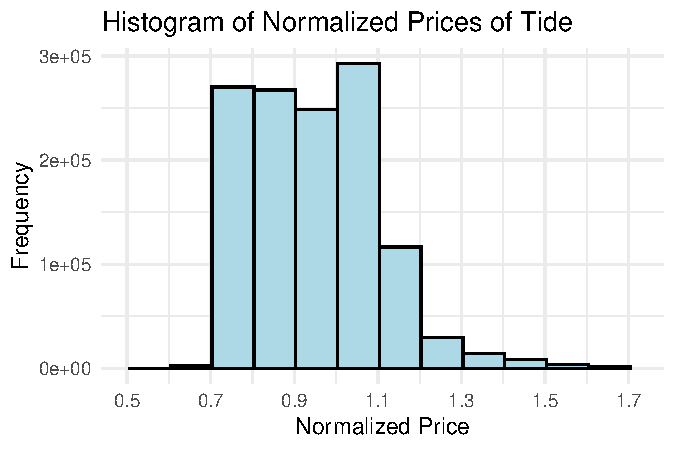
\includegraphics{Base-Pricing_files/figure-latex/unnamed-chunk-17-1} \end{flushright}

\begin{Shaded}
\begin{Highlighting}[]
\NormalTok{gain\_average }\OtherTok{=}\NormalTok{ final\_data\_with\_store[, }\FunctionTok{mean}\NormalTok{(price\_Gain, }\AttributeTok{na.rm =} \ConstantTok{TRUE}\NormalTok{)]}
\NormalTok{norm\_gain }\OtherTok{=}\NormalTok{ final\_data\_with\_store[, price\_Gain }\SpecialCharTok{/}\NormalTok{ gain\_average]}

\NormalTok{df\_gain }\OtherTok{=} \FunctionTok{data.frame}\NormalTok{(norm\_gain)}

\FunctionTok{ggplot}\NormalTok{(df\_gain, }\FunctionTok{aes}\NormalTok{(}\AttributeTok{x =}\NormalTok{ norm\_gain)) }\SpecialCharTok{+} 
  \FunctionTok{geom\_histogram}\NormalTok{(}\AttributeTok{binwidth =} \FloatTok{0.1}\NormalTok{, }\AttributeTok{fill =} \StringTok{"lightblue"}\NormalTok{, }\AttributeTok{color =} \StringTok{"black"}\NormalTok{) }\SpecialCharTok{+}
  \FunctionTok{scale\_x\_continuous}\NormalTok{(}\AttributeTok{breaks =} \FunctionTok{seq}\NormalTok{(}\FunctionTok{min}\NormalTok{(df\_gain}\SpecialCharTok{$}\NormalTok{norm\_gain, }\AttributeTok{na.rm =} \ConstantTok{TRUE}\NormalTok{), }\FunctionTok{max}\NormalTok{(df\_gain}\SpecialCharTok{$}\NormalTok{norm\_gain, }\AttributeTok{na.rm =} \ConstantTok{TRUE}\NormalTok{), }\AttributeTok{by =} \FloatTok{0.2}\NormalTok{), }
                     \AttributeTok{labels =}\NormalTok{ scales}\SpecialCharTok{::}\FunctionTok{number\_format}\NormalTok{(}\AttributeTok{accuracy =} \FloatTok{0.1}\NormalTok{)) }\SpecialCharTok{+}
  \FunctionTok{labs}\NormalTok{(}\AttributeTok{title =} \StringTok{"Histogram of Normalized Prices of Gain"}\NormalTok{, }
       \AttributeTok{x =} \StringTok{"Normalized Price"}\NormalTok{, }
       \AttributeTok{y =} \StringTok{"Frequency"}\NormalTok{) }\SpecialCharTok{+}
  \FunctionTok{theme\_minimal}\NormalTok{()}
\end{Highlighting}
\end{Shaded}

\begin{flushright}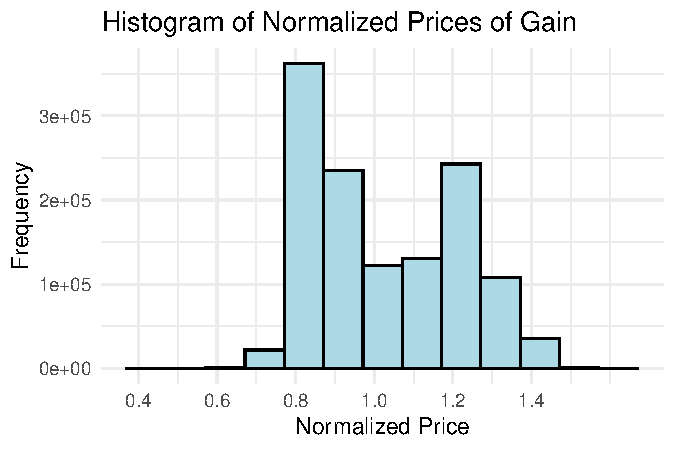
\includegraphics{Base-Pricing_files/figure-latex/unnamed-chunk-17-2} \end{flushright}

\begin{itemize}
\tightlist
\item
  \emph{To visualize relative prices, calculate the ratio of Tide and
  Gain prices with respect to the three competing brands, and show the
  histogram of relative prices.}
\end{itemize}

Note: To avoid that the scale of a graph is distorted by a few outliers,
use the \texttt{limits} option in \texttt{scale\_x\_continuous} (see the
ggplot2 introduction). This also helps to make the graphs comparable
with each other.

\begin{Shaded}
\begin{Highlighting}[]
\NormalTok{df\_tide }\OtherTok{=}\NormalTok{ final\_data\_with\_store[, .(}
  \AttributeTok{norm\_tide =}\NormalTok{ price\_Tide }\SpecialCharTok{/}\NormalTok{ ((price\_ArmHammer }\SpecialCharTok{+}\NormalTok{ price\_Purex }\SpecialCharTok{+}\NormalTok{ price\_Gain) }\SpecialCharTok{/} \DecValTok{3}\NormalTok{)}
\NormalTok{), by }\OtherTok{=}\NormalTok{ week\_end]}

\NormalTok{x\_limits }\OtherTok{=} \FunctionTok{quantile}\NormalTok{(df\_tide}\SpecialCharTok{$}\NormalTok{norm\_tide, }\AttributeTok{probs =} \FunctionTok{c}\NormalTok{(}\FloatTok{0.00}\NormalTok{, }\FloatTok{0.997}\NormalTok{), }\AttributeTok{na.rm =} \ConstantTok{TRUE}\NormalTok{)}

\FunctionTok{ggplot}\NormalTok{(df\_tide, }\FunctionTok{aes}\NormalTok{(}\AttributeTok{x =}\NormalTok{ norm\_tide)) }\SpecialCharTok{+} 
  \FunctionTok{geom\_histogram}\NormalTok{(}\AttributeTok{binwidth =} \FloatTok{0.1}\NormalTok{, }\AttributeTok{fill =} \StringTok{"lightblue"}\NormalTok{, }\AttributeTok{color =} \StringTok{"black"}\NormalTok{) }\SpecialCharTok{+}
  \FunctionTok{scale\_x\_continuous}\NormalTok{(}\AttributeTok{limits =}\NormalTok{ x\_limits) }\SpecialCharTok{+}
  \FunctionTok{labs}\NormalTok{(}\AttributeTok{title =} \StringTok{"Histogram of Relative Prices of Tide"}\NormalTok{,}
       \AttributeTok{x =} \StringTok{"Relative Price of Tide (Tide / Avg Competitors)"}\NormalTok{,}
       \AttributeTok{y =} \StringTok{"Frequency"}\NormalTok{) }\SpecialCharTok{+}
  \FunctionTok{theme\_minimal}\NormalTok{()}
\end{Highlighting}
\end{Shaded}

\begin{verbatim}
Warning: Removed 3779 rows containing non-finite outside the scale range
(`stat_bin()`).
\end{verbatim}

\begin{verbatim}
Warning: Removed 2 rows containing missing values or values outside the scale range
(`geom_bar()`).
\end{verbatim}

\begin{flushright}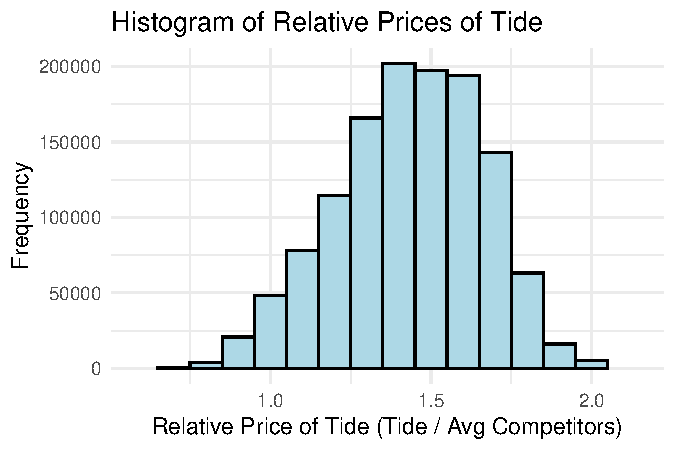
\includegraphics{Base-Pricing_files/figure-latex/unnamed-chunk-18-1} \end{flushright}

\begin{Shaded}
\begin{Highlighting}[]
\NormalTok{df\_gain }\OtherTok{=}\NormalTok{ final\_data\_with\_store[, .(}
  \AttributeTok{norm\_ggin =}\NormalTok{ price\_Gain }\SpecialCharTok{/}\NormalTok{ ((price\_ArmHammer }\SpecialCharTok{+}\NormalTok{ price\_Purex }\SpecialCharTok{+}\NormalTok{ price\_Tide) }\SpecialCharTok{/} \DecValTok{3}\NormalTok{)}
\NormalTok{), by }\OtherTok{=}\NormalTok{ week\_end]}

\FunctionTok{ggplot}\NormalTok{(df\_gain, }\FunctionTok{aes}\NormalTok{(}\AttributeTok{x =}\NormalTok{ norm\_gain)) }\SpecialCharTok{+} 
  \FunctionTok{geom\_histogram}\NormalTok{(}\AttributeTok{binwidth =} \FloatTok{0.1}\NormalTok{, }\AttributeTok{fill =} \StringTok{"lightblue"}\NormalTok{, }\AttributeTok{color =} \StringTok{"black"}\NormalTok{) }\SpecialCharTok{+}
  \FunctionTok{labs}\NormalTok{(}\AttributeTok{title =} \StringTok{"Histogram of Relative Prices of Gain"}\NormalTok{,}
       \AttributeTok{x =} \StringTok{"Relative Price of Gain (Gain / Avg Competitors)"}\NormalTok{,}
       \AttributeTok{y =} \StringTok{"Frequency"}\NormalTok{) }\SpecialCharTok{+}
  \FunctionTok{theme\_minimal}\NormalTok{()}
\end{Highlighting}
\end{Shaded}

\begin{flushright}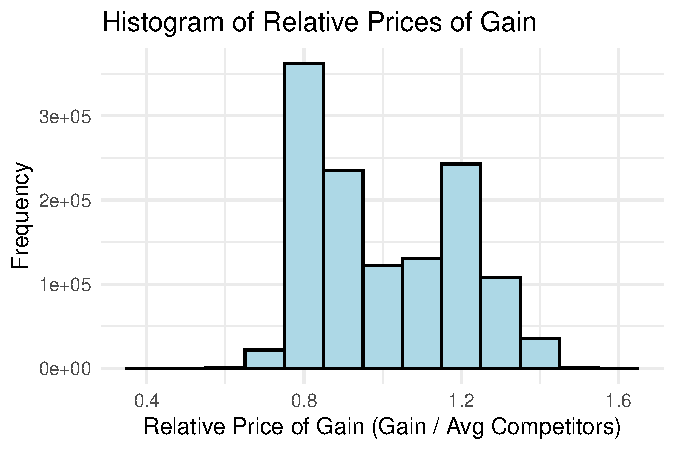
\includegraphics{Base-Pricing_files/figure-latex/unnamed-chunk-18-2} \end{flushright}

\subsection{Summary of data
inspection}\label{summary-of-data-inspection}

\emph{Discuss the data description, including sample size, geographic
coverage, and the results on own and relative price variation.}.

From having visualized the provided data, we are able to determine that
the largest single market in terms of number of observations, is Los
Angeles, with 127 244 unique instances. This is followed by Chicago and
Miami, with 88 257 and 56 504 observations respectively.

In terms of own price variation over time, we can see two very different
graphs for Tide and Gain products. The graph of the normalized price
variation of Tide tells us that for the majority of the time, the price
of the product is (mostly) evenly distributed between 70\% and 110\% of
the average price, with most instances of the product being priced
between 100-110\% of the average price. This stands in contrast to Gain
products, who display a bimodal distribution, with the majority of
prices being between 75\%-95\%, and 115\%-125\% of the average price.
The most common price was around 80\% of the average price.

Controlling for the prices of three competitors, Tide product prices
were close to normally distributed around 135-140\% of their
competitors' prices. In contrast, Gain displayed a bimodal distribution
with peaks centered at the 80\% and 120\% of competitors' prices.

\newpage

\section{Estimation}\label{estimation}

Now we are ready to estimate demand models for Tide and Gain.

We want to estimate a sequence of models with an increasing number of
controls and compare the stability of the key results across these
models. In all models the output is
\texttt{log(1+quantity\_\textless{}brand\ name\textgreater{})}.

\bigskip

To keep things simple, we will initially estimate demand for Tide only.

Let's start with the following models:

\begin{enumerate}
\def\labelenumi{\arabic{enumi}.}
\tightlist
\item
  log of own price as only input
\item
  Add store fixed effects
\item
  Add a time trend---maybe linear, or a polynomial with higher-order
  terms
\item
  Instead of a time trend add fixed effects for each month (more
  precisely: for each year/month combination)
\end{enumerate}

\emph{Estimate the models using the \texttt{feols} function from the
fixest package (consult the corresponding fixest guide included among
the R learning resources on Canvas). Store the regression outputs in
some appropriately named variables (objects).}

\begin{Shaded}
\begin{Highlighting}[]
\FunctionTok{head}\NormalTok{(final\_data\_with\_store)}
\end{Highlighting}
\end{Shaded}

\begin{verbatim}
Key: <store_code_uc>
   store_code_uc   week_end quantity_ArmHammer quantity_Gain quantity_Purex
           <int>     <Date>              <num>         <num>          <num>
1:          1123 2010-01-09               3300           700           1582
2:          1123 2010-01-16               1500           600           4988
3:          1123 2010-01-23               1275          1300            832
4:          1123 2010-01-30               4025           300           1142
5:          1123 2010-02-06               2275           300           1786
6:          1123 2010-02-13               1600             0           1288
   quantity_Tide price_ArmHammer price_Gain price_Purex price_Tide
           <num>           <num>      <num>       <num>      <num>
1:          9600      0.06852484  0.1209109  0.08248828  0.1299496
2:          3450      0.07700768  0.1209109  0.06126852  0.1519637
3:          2700      0.07757468  0.1015777  0.08214914  0.1524072
4:          2100      0.06442845  0.1209109  0.08214914  0.1524981
5:          3300      0.07757468  0.1209109  0.08214914  0.1519637
6:          6100      0.07757468  0.1209109  0.08214914  0.1303309
   promotion_ArmHammer promotion_Gain promotion_Purex promotion_Tide
                 <num>          <num>           <num>          <num>
1:                   1              0               0              1
2:                   0              0               1              0
3:                   0              1               0              0
4:                   1              0               0              0
5:                   0              0               0              0
6:                   0              0               0              1
   retailer_code store_zip3 SMM_code SMM_description  year month month_trend
           <int>      <int>    <int>          <char> <num> <num>       <num>
1:            89        441       16       Cleveland  2010     1           1
2:            89        441       16       Cleveland  2010     1           1
3:            89        441       16       Cleveland  2010     1           1
4:            89        441       16       Cleveland  2010     1           1
5:            89        441       16       Cleveland  2010     2           2
6:            89        441       16       Cleveland  2010     2           2
\end{verbatim}

\begin{Shaded}
\begin{Highlighting}[]
\NormalTok{fit\_base }\OtherTok{\textless{}{-}} \FunctionTok{feols}\NormalTok{(}
  \FunctionTok{log}\NormalTok{(}\DecValTok{1} \SpecialCharTok{+}\NormalTok{ quantity\_Tide) }\SpecialCharTok{\textasciitilde{}} \FunctionTok{log}\NormalTok{(price\_Tide),}
  \AttributeTok{data =}\NormalTok{ final\_data\_with\_store}
\NormalTok{)}

\NormalTok{fit\_store\_FE }\OtherTok{\textless{}{-}} \FunctionTok{feols}\NormalTok{(}
  \FunctionTok{log}\NormalTok{(}\DecValTok{1} \SpecialCharTok{+}\NormalTok{ quantity\_Tide) }\SpecialCharTok{\textasciitilde{}} \FunctionTok{log}\NormalTok{(price\_Tide) }\SpecialCharTok{|}\NormalTok{ store\_code\_uc,}
  \AttributeTok{data =}\NormalTok{ final\_data\_with\_store}
\NormalTok{)}

\NormalTok{fit\_trend }\OtherTok{\textless{}{-}} \FunctionTok{feols}\NormalTok{(}
  \FunctionTok{log}\NormalTok{(}\DecValTok{1} \SpecialCharTok{+}\NormalTok{ quantity\_Tide) }\SpecialCharTok{\textasciitilde{}} \FunctionTok{log}\NormalTok{(price\_Tide) }\SpecialCharTok{+}\NormalTok{ month }\SpecialCharTok{|}\NormalTok{ store\_code\_uc,}
  \AttributeTok{data =}\NormalTok{ final\_data\_with\_store}
\NormalTok{)}

\NormalTok{fit\_month\_FE }\OtherTok{\textless{}{-}} \FunctionTok{feols}\NormalTok{(}
  \FunctionTok{log}\NormalTok{(}\DecValTok{1} \SpecialCharTok{+}\NormalTok{ quantity\_Tide) }\SpecialCharTok{\textasciitilde{}} \FunctionTok{log}\NormalTok{(price\_Tide) }\SpecialCharTok{|}\NormalTok{ store\_code\_uc }\SpecialCharTok{+}\NormalTok{ year }\SpecialCharTok{+}\NormalTok{ month,}
  \AttributeTok{data =}\NormalTok{ final\_data\_with\_store}
\NormalTok{)}

\NormalTok{fit\_promo\_Tide }\OtherTok{\textless{}{-}} \FunctionTok{feols}\NormalTok{(}
  \FunctionTok{log}\NormalTok{(}\DecValTok{1} \SpecialCharTok{+}\NormalTok{ quantity\_Tide) }\SpecialCharTok{\textasciitilde{}} \FunctionTok{log}\NormalTok{(price\_Tide) }\SpecialCharTok{+} 
\NormalTok{    promotion\_Tide }\SpecialCharTok{|}\NormalTok{ store\_code\_uc }\SpecialCharTok{+}\NormalTok{ year }\SpecialCharTok{+}\NormalTok{ month,}
  \AttributeTok{data =}\NormalTok{ final\_data\_with\_store}
\NormalTok{)}

\FunctionTok{etable}\NormalTok{(fit\_base, fit\_store\_FE, fit\_trend, fit\_month\_FE, fit\_promo\_Tide)}
\end{Highlighting}
\end{Shaded}

\begin{verbatim}
                            fit_base         fit_store_FE            fit_trend
Dependent Var.: log(1+quantity_Tide) log(1+quantity_Tide) log(1+quantity_Tide)
                                                                              
Constant          -6.374*** (0.0127)                                          
log(price_Tide)   -7.465*** (0.0067)   -5.612*** (0.0440)   -5.607*** (0.0440)
month                                                      -0.0101*** (0.0002)
promotion_Tide                                                                
Fixed-Effects:  -------------------- -------------------- --------------------
store_code_uc                     No                  Yes                  Yes
year                              No                   No                   No
month                             No                   No                   No
_______________ ____________________ ____________________ ____________________
S.E. type                        IID    by: store_code_uc    by: store_code_uc
Observations               1,259,352            1,259,352            1,259,352
R2                           0.49632              0.84607              0.84652
Within R2                         --              0.29829              0.30034

                        fit_month_FE       fit_promo_Tide
Dependent Var.: log(1+quantity_Tide) log(1+quantity_Tide)
                                                         
Constant                                                 
log(price_Tide)   -5.647*** (0.0440)   -4.076*** (0.0541)
month                                                    
promotion_Tide                         0.3665*** (0.0078)
Fixed-Effects:  -------------------- --------------------
store_code_uc                    Yes                  Yes
year                             Yes                  Yes
month                            Yes                  Yes
_______________ ____________________ ____________________
S.E. type          by: store_code_uc    by: store_code_uc
Observations               1,259,352            1,259,352
R2                           0.85144              0.85703
Within R2                    0.30448              0.33064
---
Signif. codes: 0 '***' 0.001 '**' 0.01 '*' 0.05 '.' 0.1 ' ' 1
\end{verbatim}

\bigskip

\textbf{Hint}: Recall that it is perfectly legitimate in R to write
model formulas such as

\begin{verbatim}
log(1+quantity_<brand name>) ~ log(price_<brand name>)
\end{verbatim}

Hence, there is no need to create new variables such as the logarithm of
own price, etc., before estimating a demand model.

\bigskip

You can display the regression coefficients using the \texttt{summary}
function. As a much more elegant solution, however, I recommend using
the \texttt{etable} function in the \texttt{fixest} package, which
produces nicely formatted output.

Please \textbf{consult the fixest guide on how to use \texttt{etable}},
and \textbf{go through the} \textbf{\emph{Checklist for creating LaTeX
tables using \texttt{etable}}}!

Here is an example (note that the \texttt{fit} objects are the
regression outputs---adjust the names if necessary):

\begin{Shaded}
\begin{Highlighting}[]
\CommentTok{\#etable(fit\_base, fit\_store\_FE, fit\_trend, fit\_month\_FE,}
       \CommentTok{\#tex = TRUE,}
       \CommentTok{\#fitstat = c("n", "r2"), signif.code = NA,}
       \CommentTok{\#cluster = c("store\_code\_uc", "month\_trend"))}
\end{Highlighting}
\end{Shaded}

Note the option
\texttt{cluster\ =\ c("store\_code\_uc",\ "month\_trend")}, which tells
\texttt{etable} to show standard errors that are clustered at the store
and month level. These clustered standard errors will be larger and more
accurate than regular standard errors because they reflect that the
error terms in the regression are likely correlated at the store and
month level.

\bigskip

Before moving on, you may want to remove the regression output objects
that are no longer used, because they take up much space in memory:

\begin{Shaded}
\begin{Highlighting}[]
\FunctionTok{rm}\NormalTok{(fit\_base, fit\_store\_FE, fit\_trend)}
\end{Highlighting}
\end{Shaded}

\subsection{Controlling for competitor
prices}\label{controlling-for-competitor-prices}

\emph{Now add the competitor prices to the demand model.}

\begin{Shaded}
\begin{Highlighting}[]
\FunctionTok{library}\NormalTok{(fixest)}

\NormalTok{fit\_base\_competitor }\OtherTok{\textless{}{-}} \FunctionTok{feols}\NormalTok{(}
  \FunctionTok{log}\NormalTok{(}\DecValTok{1} \SpecialCharTok{+}\NormalTok{ quantity\_Tide) }\SpecialCharTok{\textasciitilde{}} \FunctionTok{log}\NormalTok{(price\_Tide) }\SpecialCharTok{+} \FunctionTok{log}\NormalTok{(price\_Gain),}
  \AttributeTok{data =}\NormalTok{ final\_data\_with\_store}
\NormalTok{)}

\NormalTok{fit\_store\_FE\_competitor }\OtherTok{\textless{}{-}} \FunctionTok{feols}\NormalTok{(}
  \FunctionTok{log}\NormalTok{(}\DecValTok{1} \SpecialCharTok{+}\NormalTok{ quantity\_Tide) }\SpecialCharTok{\textasciitilde{}} \FunctionTok{log}\NormalTok{(price\_Tide) }\SpecialCharTok{+} \FunctionTok{log}\NormalTok{(price\_Gain) }\SpecialCharTok{+}
    \FunctionTok{log}\NormalTok{(price\_ArmHammer) }\SpecialCharTok{+} \FunctionTok{log}\NormalTok{(price\_Purex) }\SpecialCharTok{|}\NormalTok{ store\_code\_uc,}
  \AttributeTok{data =}\NormalTok{ final\_data\_with\_store}
\NormalTok{)}

\NormalTok{fit\_trend\_competitor }\OtherTok{\textless{}{-}} \FunctionTok{feols}\NormalTok{(}
  \FunctionTok{log}\NormalTok{(}\DecValTok{1} \SpecialCharTok{+}\NormalTok{ quantity\_Tide) }\SpecialCharTok{\textasciitilde{}} \FunctionTok{log}\NormalTok{(price\_Tide) }\SpecialCharTok{+} \FunctionTok{log}\NormalTok{(price\_Gain) }\SpecialCharTok{+} 
    \FunctionTok{log}\NormalTok{(price\_ArmHammer) }\SpecialCharTok{+} \FunctionTok{log}\NormalTok{(price\_Purex) }\SpecialCharTok{+}\NormalTok{ month }\SpecialCharTok{|}\NormalTok{ store\_code\_uc, }
  \AttributeTok{data =}\NormalTok{ final\_data\_with\_store}
\NormalTok{)}

\NormalTok{fit\_month\_FE\_competitor }\OtherTok{\textless{}{-}} \FunctionTok{feols}\NormalTok{(}
  \FunctionTok{log}\NormalTok{(}\DecValTok{1} \SpecialCharTok{+}\NormalTok{ quantity\_Tide) }\SpecialCharTok{\textasciitilde{}} \FunctionTok{log}\NormalTok{(price\_Tide) }\SpecialCharTok{+} \FunctionTok{log}\NormalTok{(price\_Gain) }\SpecialCharTok{+} 
    \FunctionTok{log}\NormalTok{(price\_ArmHammer) }\SpecialCharTok{+} \FunctionTok{log}\NormalTok{(price\_Purex) }\SpecialCharTok{|}\NormalTok{ store\_code\_uc }\SpecialCharTok{+}\NormalTok{ year }\SpecialCharTok{+}\NormalTok{ month, }
  \AttributeTok{data =}\NormalTok{ final\_data\_with\_store)}

\FunctionTok{etable}\NormalTok{(fit\_base\_competitor, fit\_store\_FE\_competitor, fit\_trend\_competitor,}
\NormalTok{       fit\_month\_FE\_competitor)}
\end{Highlighting}
\end{Shaded}

\begin{verbatim}
                      fit_base_competitor fit_store_FE_compe..
Dependent Var.:      log(1+quantity_Tide) log(1+quantity_Tide)
                                                              
Constant               -7.559*** (0.0128)                     
log(price_Tide)        -5.792*** (0.0084)   -5.639*** (0.0436)
log(price_Gain)        -2.126*** (0.0068)   0.7171*** (0.0180)
log(price_ArmHammer)                        0.1360*** (0.0052)
log(price_Purex)                           -0.0544*** (0.0054)
month                                                         
Fixed-Effects:       -------------------- --------------------
store_code_uc                          No                  Yes
year                                   No                   No
month                                  No                   No
____________________ ____________________ ____________________
S.E. type                             IID    by: store_code_uc
Observations                    1,259,352            1,259,352
R2                                0.53281              0.84867
Within R2                              --              0.31013

                     fit_trend_competitor fit_month_FE_compe..
Dependent Var.:      log(1+quantity_Tide) log(1+quantity_Tide)
                                                              
Constant                                                      
log(price_Tide)        -5.636*** (0.0435)   -5.643*** (0.0430)
log(price_Gain)        0.7075*** (0.0181)   0.6279*** (0.0188)
log(price_ArmHammer)   0.1229*** (0.0051)   0.1048*** (0.0050)
log(price_Purex)      -0.0495*** (0.0054)   0.1565*** (0.0075)
month                 -0.0083*** (0.0002)                     
Fixed-Effects:       -------------------- --------------------
store_code_uc                         Yes                  Yes
year                                   No                  Yes
month                                  No                  Yes
____________________ ____________________ ____________________
S.E. type               by: store_code_uc    by: store_code_uc
Observations                    1,259,352            1,259,352
R2                                0.84896              0.85368
Within R2                         0.31148              0.31498
---
Signif. codes: 0 '***' 0.001 '**' 0.01 '*' 0.05 '.' 0.1 ' ' 1
\end{verbatim}

\subsection{Controlling for
promotions}\label{controlling-for-promotions}

\emph{Now add the promotions dummies, first just for Tide, then for all
brands. Compare the results. Did controlling for promotions change the
own price elasticity estimate in an expected manner?}

\begin{Shaded}
\begin{Highlighting}[]
\CommentTok{\#Tide}

\NormalTok{fit\_base\_competitor\_promo }\OtherTok{\textless{}{-}} \FunctionTok{feols}\NormalTok{(}
  \FunctionTok{log}\NormalTok{(}\DecValTok{1} \SpecialCharTok{+}\NormalTok{ quantity\_Tide) }\SpecialCharTok{\textasciitilde{}} \FunctionTok{log}\NormalTok{(price\_Tide) }\SpecialCharTok{+} \FunctionTok{log}\NormalTok{(price\_Gain) }\SpecialCharTok{+}
    \FunctionTok{log}\NormalTok{(price\_ArmHammer) }\SpecialCharTok{+} \FunctionTok{log}\NormalTok{(price\_Purex) }\SpecialCharTok{+}\NormalTok{ promotion\_Tide,}
  \AttributeTok{data =}\NormalTok{ final\_data\_with\_store}
\NormalTok{)}

\NormalTok{fit\_store\_FE\_competitor\_promo }\OtherTok{\textless{}{-}} \FunctionTok{feols}\NormalTok{(}
  \FunctionTok{log}\NormalTok{(}\DecValTok{1} \SpecialCharTok{+}\NormalTok{ quantity\_Tide) }\SpecialCharTok{\textasciitilde{}} \FunctionTok{log}\NormalTok{(price\_Tide) }\SpecialCharTok{+} \FunctionTok{log}\NormalTok{(price\_Gain) }\SpecialCharTok{+}
    \FunctionTok{log}\NormalTok{(price\_ArmHammer) }\SpecialCharTok{+} \FunctionTok{log}\NormalTok{(price\_Purex) }\SpecialCharTok{+}\NormalTok{ promotion\_Tide }\SpecialCharTok{|}\NormalTok{ store\_code\_uc,}
  \AttributeTok{data =}\NormalTok{ final\_data\_with\_store}
\NormalTok{)}

\NormalTok{fit\_trend\_competitor\_promo }\OtherTok{\textless{}{-}} \FunctionTok{feols}\NormalTok{(}
  \FunctionTok{log}\NormalTok{(}\DecValTok{1} \SpecialCharTok{+}\NormalTok{ quantity\_Tide) }\SpecialCharTok{\textasciitilde{}} \FunctionTok{log}\NormalTok{(price\_Tide) }\SpecialCharTok{+} \FunctionTok{log}\NormalTok{(price\_Gain) }\SpecialCharTok{+} 
    \FunctionTok{log}\NormalTok{(price\_ArmHammer) }\SpecialCharTok{+} \FunctionTok{log}\NormalTok{(price\_Purex) }\SpecialCharTok{+}\NormalTok{ month }\SpecialCharTok{+} 
\NormalTok{    promotion\_Tide }\SpecialCharTok{|}\NormalTok{ store\_code\_uc,}
  \AttributeTok{data =}\NormalTok{ final\_data\_with\_store}
\NormalTok{)}

\NormalTok{fit\_month\_FE\_competitor\_promo }\OtherTok{\textless{}{-}} \FunctionTok{feols}\NormalTok{(}
  \FunctionTok{log}\NormalTok{(}\DecValTok{1} \SpecialCharTok{+}\NormalTok{ quantity\_Tide) }\SpecialCharTok{\textasciitilde{}} \FunctionTok{log}\NormalTok{(price\_Tide) }\SpecialCharTok{+} \FunctionTok{log}\NormalTok{(price\_Gain) }\SpecialCharTok{+} 
    \FunctionTok{log}\NormalTok{(price\_ArmHammer) }\SpecialCharTok{+} \FunctionTok{log}\NormalTok{(price\_Purex) }\SpecialCharTok{+} 
\NormalTok{    promotion\_Tide }\SpecialCharTok{|}\NormalTok{ store\_code\_uc }\SpecialCharTok{+}\NormalTok{ year }\SpecialCharTok{+}\NormalTok{ month,}
  \AttributeTok{data =}\NormalTok{ final\_data\_with\_store}
\NormalTok{)}

\FunctionTok{etable}\NormalTok{(fit\_base\_competitor\_promo, fit\_store\_FE\_competitor\_promo, }
\NormalTok{       fit\_trend\_competitor\_promo, fit\_month\_FE\_competitor\_promo)}
\end{Highlighting}
\end{Shaded}

\begin{verbatim}
                     fit_base_competito.. fit_store_FE_compe..
Dependent Var.:      log(1+quantity_Tide) log(1+quantity_Tide)
                                                              
Constant               -7.072*** (0.0129)                     
log(price_Tide)        -4.127*** (0.0096)   -3.971*** (0.0527)
log(price_Gain)        -1.770*** (0.0075)   0.5498*** (0.0177)
log(price_ArmHammer)   -1.111*** (0.0039)   0.0931*** (0.0051)
log(price_Purex)      -0.2270*** (0.0029)  -0.0422*** (0.0048)
promotion_Tide         0.4755*** (0.0023)   0.3907*** (0.0080)
month                                                         
Fixed-Effects:       -------------------- --------------------
store_code_uc                          No                  Yes
year                                   No                   No
month                                  No                   No
____________________ ____________________ ____________________
S.E. type                             IID    by: store_code_uc
Observations                    1,259,352            1,259,352
R2                                0.56996              0.85513
Within R2                              --              0.33962

                     fit_trend_competit.. fit_month_FE_compe..
Dependent Var.:      log(1+quantity_Tide) log(1+quantity_Tide)
                                                              
Constant                                                      
log(price_Tide)        -3.985*** (0.0528)   -4.180*** (0.0548)
log(price_Gain)        0.5448*** (0.0178)   0.4990*** (0.0185)
log(price_ArmHammer)   0.0843*** (0.0051)   0.0753*** (0.0049)
log(price_Purex)      -0.0389*** (0.0048)   0.1315*** (0.0071)
promotion_Tide         0.3869*** (0.0080)   0.3416*** (0.0077)
month                 -0.0058*** (0.0002)                     
Fixed-Effects:       -------------------- --------------------
store_code_uc                         Yes                  Yes
year                                   No                  Yes
month                                  No                  Yes
____________________ ____________________ ____________________
S.E. type               by: store_code_uc    by: store_code_uc
Observations                    1,259,352            1,259,352
R2                                0.85528              0.85844
Within R2                         0.34028              0.33727
---
Signif. codes: 0 '***' 0.001 '**' 0.01 '*' 0.05 '.' 0.1 ' ' 1
\end{verbatim}

When comparing the models without promotions against the ones with
promotions, the latter has less own price elasticity: 3.961 (promotions)
vs 5.659 (no promotions). Without controlling for promotions, their
effect is mistakenly attributed to price, which inflates the price
elasticity. When promotions are included, the model correctly attributes
the demand increase to them, resulting in a more accurate, lower price
elasticity. This reflects the fact that consumers are less sensitive to
price changes alone than the model without promotions suggested, as
promotions are often more effective at boosting demand than small price
reductions.

\begin{Shaded}
\begin{Highlighting}[]
\CommentTok{\# All Brands}

\NormalTok{fit\_base\_competitor\_promo2 }\OtherTok{\textless{}{-}} \FunctionTok{feols}\NormalTok{(}
  \FunctionTok{log}\NormalTok{(}\DecValTok{1} \SpecialCharTok{+}\NormalTok{ quantity\_Tide) }\SpecialCharTok{\textasciitilde{}} \FunctionTok{log}\NormalTok{(price\_Tide) }\SpecialCharTok{+} \FunctionTok{log}\NormalTok{(price\_Gain) }\SpecialCharTok{+} 
    \FunctionTok{log}\NormalTok{(price\_ArmHammer) }\SpecialCharTok{+} \FunctionTok{log}\NormalTok{(price\_Purex) }\SpecialCharTok{+}\NormalTok{ promotion\_Tide }\SpecialCharTok{+} 
\NormalTok{    promotion\_Gain }\SpecialCharTok{+}\NormalTok{ promotion\_ArmHammer }\SpecialCharTok{+}\NormalTok{ promotion\_Purex, }
  \AttributeTok{data =}\NormalTok{ final\_data\_with\_store}
\NormalTok{)}

\NormalTok{fit\_store\_FE\_competitor\_promo2 }\OtherTok{\textless{}{-}} \FunctionTok{feols}\NormalTok{(}
  \FunctionTok{log}\NormalTok{(}\DecValTok{1} \SpecialCharTok{+}\NormalTok{ quantity\_Tide) }\SpecialCharTok{\textasciitilde{}} \FunctionTok{log}\NormalTok{(price\_Tide) }\SpecialCharTok{+} \FunctionTok{log}\NormalTok{(price\_Gain) }\SpecialCharTok{+}
    \FunctionTok{log}\NormalTok{(price\_ArmHammer) }\SpecialCharTok{+} \FunctionTok{log}\NormalTok{(price\_Purex) }\SpecialCharTok{+}\NormalTok{ promotion\_Tide }\SpecialCharTok{+} 
\NormalTok{    promotion\_Gain }\SpecialCharTok{+}\NormalTok{ promotion\_ArmHammer }\SpecialCharTok{+}\NormalTok{ promotion\_Purex }\SpecialCharTok{|}\NormalTok{ store\_code\_uc, }
  \AttributeTok{data =}\NormalTok{ final\_data\_with\_store}
\NormalTok{)}

\NormalTok{fit\_trend\_competitor\_promo2 }\OtherTok{\textless{}{-}} \FunctionTok{feols}\NormalTok{(}
  \FunctionTok{log}\NormalTok{(}\DecValTok{1} \SpecialCharTok{+}\NormalTok{ quantity\_Tide) }\SpecialCharTok{\textasciitilde{}} \FunctionTok{log}\NormalTok{(price\_Tide) }\SpecialCharTok{+} \FunctionTok{log}\NormalTok{(price\_Gain) }\SpecialCharTok{+} 
    \FunctionTok{log}\NormalTok{(price\_ArmHammer) }\SpecialCharTok{+} \FunctionTok{log}\NormalTok{(price\_Purex) }\SpecialCharTok{+}\NormalTok{ month }\SpecialCharTok{+} 
\NormalTok{    promotion\_Tide }\SpecialCharTok{+}\NormalTok{ promotion\_Gain }\SpecialCharTok{+}\NormalTok{ promotion\_ArmHammer }\SpecialCharTok{+}\NormalTok{ promotion\_Purex }\SpecialCharTok{|} 
\NormalTok{    store\_code\_uc, }\AttributeTok{data =}\NormalTok{ final\_data\_with\_store}
\NormalTok{)}

\NormalTok{fit\_month\_FE\_competitor\_promo2 }\OtherTok{\textless{}{-}} \FunctionTok{feols}\NormalTok{(}
  \FunctionTok{log}\NormalTok{(}\DecValTok{1} \SpecialCharTok{+}\NormalTok{ quantity\_Tide) }\SpecialCharTok{\textasciitilde{}} \FunctionTok{log}\NormalTok{(price\_Tide) }\SpecialCharTok{+} \FunctionTok{log}\NormalTok{(price\_Gain) }\SpecialCharTok{+} 
    \FunctionTok{log}\NormalTok{(price\_ArmHammer) }\SpecialCharTok{+} \FunctionTok{log}\NormalTok{(price\_Purex) }\SpecialCharTok{+}\NormalTok{ promotion\_Tide }\SpecialCharTok{+} 
\NormalTok{    promotion\_Gain }\SpecialCharTok{+}\NormalTok{ promotion\_ArmHammer }\SpecialCharTok{+}\NormalTok{ promotion\_Purex }\SpecialCharTok{|}\NormalTok{ store\_code\_uc }\SpecialCharTok{+} 
\NormalTok{    year }\SpecialCharTok{+}\NormalTok{ month, }\AttributeTok{data =}\NormalTok{ final\_data\_with\_store}
\NormalTok{)}

\FunctionTok{etable}\NormalTok{(fit\_base\_competitor\_promo2, fit\_store\_FE\_competitor\_promo2, }
\NormalTok{       fit\_trend\_competitor\_promo2, fit\_month\_FE\_competitor\_promo2)}
\end{Highlighting}
\end{Shaded}

\begin{verbatim}
                     fit_base_competit..2 fit_store_FE_comp..2
Dependent Var.:      log(1+quantity_Tide) log(1+quantity_Tide)
                                                              
Constant               -6.583*** (0.0131)                     
log(price_Tide)        -3.307*** (0.0100)   -4.003*** (0.0531)
log(price_Gain)        -2.273*** (0.0090)   0.6922*** (0.0238)
log(price_ArmHammer)   -1.210*** (0.0049)   0.1437*** (0.0092)
log(price_Purex)      -0.2223*** (0.0031)  -0.0661*** (0.0060)
promotion_Tide         0.5647*** (0.0023)   0.3832*** (0.0082)
promotion_Gain        -0.4755*** (0.0029)   0.0577*** (0.0060)
promotion_ArmHammer   -0.2909*** (0.0024)   0.0331*** (0.0062)
promotion_Purex       -0.0807*** (0.0021)  -0.0404*** (0.0050)
month                                                         
Fixed-Effects:       -------------------- --------------------
store_code_uc                          No                  Yes
year                                   No                   No
month                                  No                   No
____________________ ____________________ ____________________
S.E. type                             IID    by: store_code_uc
Observations                    1,259,352            1,259,352
R2                                0.58840              0.85540
Within R2                              --              0.34084

                     fit_trend_competi..2 fit_month_FE_comp..2
Dependent Var.:      log(1+quantity_Tide) log(1+quantity_Tide)
                                                              
Constant                                                      
log(price_Tide)        -4.015*** (0.0532)   -4.196*** (0.0549)
log(price_Gain)        0.6830*** (0.0238)   0.5748*** (0.0242)
log(price_ArmHammer)   0.1325*** (0.0092)   0.1223*** (0.0087)
log(price_Purex)      -0.0624*** (0.0060)   0.1515*** (0.0129)
promotion_Tide         0.3799*** (0.0082)   0.3411*** (0.0077)
promotion_Gain         0.0559*** (0.0060)   0.0314*** (0.0053)
promotion_ArmHammer    0.0311*** (0.0062)   0.0346*** (0.0059)
promotion_Purex       -0.0394*** (0.0050)    0.0222** (0.0072)
month                 -0.0054*** (0.0002)                     
Fixed-Effects:       -------------------- --------------------
store_code_uc                         Yes                  Yes
year                                   No                  Yes
month                                  No                  Yes
____________________ ____________________ ____________________
S.E. type               by: store_code_uc    by: store_code_uc
Observations                    1,259,352            1,259,352
R2                                0.85553              0.85856
Within R2                         0.34142              0.33782
---
Signif. codes: 0 '***' 0.001 '**' 0.01 '*' 0.05 '.' 0.1 ' ' 1
\end{verbatim}

With the exception of the fit\_base model, all other models are
generally the same compared to the models with the single promotion.

\bigskip

\emph{Summarize and comment on the estimation results. Was it necessary
to control for store fixed effects, time trends/fixed effects, as well
as competitor prices and promotions? What do we learn from the
magnitudes of the own and cross-price elasticities?}

In the base model, Tide's own-price elasticity is quite large, with a
coefficient of -7.47, indicating that a 1\% increase in Tide's price
would result in a 7.47\% decrease in demand. However, after including
store fixed effects, the magnitude of this elasticity decreases to
-5.61, suggesting that the initial model without controls overestimated
Tide's price sensitivity by failing to account for unobserved
differences across stores. The R-squared value also jumps from 0.496 in
the base model to 0.846, which demonstrates the significant improvement
in model fit when store-specific factors are considered.

Time trends and month fixed effects did not have much of an impact on
the overall results. After introducing a month trend, the price
elasticity remains at -5.61, and the inclusion of fixed effects for each
year and month leads to a slight decrease in price elasticity to -5.65.
The R-squared improves marginally to 0.851, indicating that time trends
capture some of the seasonality in Tide's demand, but store fixed
effects remain the most important control.

Lastly, the introduction of Tide's promotional activities further
improves the model's explanatory power, with the R-squared rising to
0.857. The own-price elasticity decreases further to -4.08, indicating
that promotions significantly mitigate the negative impact of price
increases. Promotions for Tide have a strong and positive effect on
sales, increasing demand by approximately 36.65\%. This confirms that
promotions are a major driver of Tide's demand and should be accounted
for when estimating price sensitivity.

\bigskip

We will use the final model including all variables (I called it
\texttt{fit\_promo\_comp}) as our preferred model. To make this final
model distinguishable from the regression output for Gain we rename it:

\begin{Shaded}
\begin{Highlighting}[]
\NormalTok{fit\_promo\_comp }\OtherTok{\textless{}{-}} \FunctionTok{feols}\NormalTok{(}
  \FunctionTok{log}\NormalTok{(}\DecValTok{1} \SpecialCharTok{+}\NormalTok{ quantity\_Tide) }\SpecialCharTok{\textasciitilde{}} \FunctionTok{log}\NormalTok{(price\_Tide) }\SpecialCharTok{+} \FunctionTok{log}\NormalTok{(price\_Gain) }\SpecialCharTok{+} \FunctionTok{log}\NormalTok{(price\_Purex)}
  \SpecialCharTok{+} \FunctionTok{log}\NormalTok{(price\_ArmHammer) }\SpecialCharTok{+}\NormalTok{ promotion\_Tide }\SpecialCharTok{+}\NormalTok{ promotion\_Gain }\SpecialCharTok{+}\NormalTok{ promotion\_ArmHammer}
  \SpecialCharTok{+}\NormalTok{ promotion\_Purex }\SpecialCharTok{|}\NormalTok{ store\_code\_uc }\SpecialCharTok{+}\NormalTok{ year }\SpecialCharTok{+}\NormalTok{ month, }\AttributeTok{data =}\NormalTok{ final\_data\_with\_store}
\NormalTok{)}
\end{Highlighting}
\end{Shaded}

\begin{Shaded}
\begin{Highlighting}[]
\NormalTok{fit\_Tide }\OtherTok{=}\NormalTok{ fit\_promo\_comp}
\end{Highlighting}
\end{Shaded}

\subsection{Demand model for Gain}\label{demand-model-for-gain}

\emph{Now repeat the steps to estimate demand for Gain.}

\begin{Shaded}
\begin{Highlighting}[]
\NormalTok{fit\_base }\OtherTok{\textless{}{-}} \FunctionTok{feols}\NormalTok{(}
  \FunctionTok{log}\NormalTok{(}\DecValTok{1} \SpecialCharTok{+}\NormalTok{ quantity\_Gain) }\SpecialCharTok{\textasciitilde{}} \FunctionTok{log}\NormalTok{(price\_Gain),}
  \AttributeTok{data =}\NormalTok{ final\_data\_with\_store}
\NormalTok{)}

\NormalTok{fit\_store\_FE }\OtherTok{\textless{}{-}} \FunctionTok{feols}\NormalTok{(}
  \FunctionTok{log}\NormalTok{(}\DecValTok{1} \SpecialCharTok{+}\NormalTok{ quantity\_Gain) }\SpecialCharTok{\textasciitilde{}} \FunctionTok{log}\NormalTok{(price\_Gain) }\SpecialCharTok{|}\NormalTok{ store\_code\_uc,}
  \AttributeTok{data =}\NormalTok{ final\_data\_with\_store}
\NormalTok{)}

\NormalTok{fit\_trend }\OtherTok{\textless{}{-}} \FunctionTok{feols}\NormalTok{(}
  \FunctionTok{log}\NormalTok{(}\DecValTok{1} \SpecialCharTok{+}\NormalTok{ quantity\_Gain) }\SpecialCharTok{\textasciitilde{}} \FunctionTok{log}\NormalTok{(price\_Gain) }\SpecialCharTok{+}\NormalTok{ month }\SpecialCharTok{|}\NormalTok{ store\_code\_uc,}
  \AttributeTok{data =}\NormalTok{ final\_data\_with\_store}
\NormalTok{)}

\NormalTok{fit\_month\_FE }\OtherTok{\textless{}{-}} \FunctionTok{feols}\NormalTok{(}
  \FunctionTok{log}\NormalTok{(}\DecValTok{1} \SpecialCharTok{+}\NormalTok{ quantity\_Gain) }\SpecialCharTok{\textasciitilde{}} \FunctionTok{log}\NormalTok{(price\_Gain) }\SpecialCharTok{|}\NormalTok{ store\_code\_uc }\SpecialCharTok{+}\NormalTok{ year }\SpecialCharTok{+}\NormalTok{ month,}
  \AttributeTok{data =}\NormalTok{ final\_data\_with\_store}
\NormalTok{)}

\NormalTok{fit\_promo\_Gain }\OtherTok{\textless{}{-}} \FunctionTok{feols}\NormalTok{(}
  \FunctionTok{log}\NormalTok{(}\DecValTok{1} \SpecialCharTok{+}\NormalTok{ quantity\_Gain) }\SpecialCharTok{\textasciitilde{}} \FunctionTok{log}\NormalTok{(price\_Gain) }\SpecialCharTok{+}\NormalTok{ promotion\_Gain }\SpecialCharTok{|}\NormalTok{ store\_code\_uc }\SpecialCharTok{+} 
\NormalTok{    year }\SpecialCharTok{+}\NormalTok{ month,}
  \AttributeTok{data =}\NormalTok{ final\_data\_with\_store}
\NormalTok{)}

\FunctionTok{etable}\NormalTok{(fit\_base, fit\_store\_FE, fit\_trend, fit\_month\_FE, fit\_promo\_Gain)}
\end{Highlighting}
\end{Shaded}

\begin{verbatim}
                            fit_base         fit_store_FE            fit_trend
Dependent Var.: log(1+quantity_Gain) log(1+quantity_Gain) log(1+quantity_Gain)
                                                                              
Constant          -14.55*** (0.0160)                                          
log(price_Gain)   -9.967*** (0.0078)   -6.709*** (0.0326)   -6.690*** (0.0326)
month                                                       0.0157*** (0.0005)
promotion_Gain                                                                
Fixed-Effects:  -------------------- -------------------- --------------------
store_code_uc                     No                  Yes                  Yes
year                              No                   No                   No
month                             No                   No                   No
_______________ ____________________ ____________________ ____________________
S.E. type                        IID    by: store_code_uc    by: store_code_uc
Observations               1,259,352            1,259,352            1,259,352
R2                           0.56615              0.74513              0.74559
Within R2                         --              0.23514              0.23651

                        fit_month_FE       fit_promo_Gain
Dependent Var.: log(1+quantity_Gain) log(1+quantity_Gain)
                                                         
Constant                                                 
log(price_Gain)   -6.626*** (0.0328)   -4.779*** (0.0417)
month                                                    
promotion_Gain                         0.7303*** (0.0121)
Fixed-Effects:  -------------------- --------------------
store_code_uc                    Yes                  Yes
year                             Yes                  Yes
month                            Yes                  Yes
_______________ ____________________ ____________________
S.E. type          by: store_code_uc    by: store_code_uc
Observations               1,259,352            1,259,352
R2                           0.74747              0.75396
Within R2                    0.22771              0.24756
---
Signif. codes: 0 '***' 0.001 '**' 0.01 '*' 0.05 '.' 0.1 ' ' 1
\end{verbatim}

\begin{Shaded}
\begin{Highlighting}[]
\FunctionTok{library}\NormalTok{(fixest)}

\NormalTok{fit\_base\_competitor }\OtherTok{\textless{}{-}} \FunctionTok{feols}\NormalTok{(}
  \FunctionTok{log}\NormalTok{(}\DecValTok{1} \SpecialCharTok{+}\NormalTok{ quantity\_Gain) }\SpecialCharTok{\textasciitilde{}} \FunctionTok{log}\NormalTok{(price\_Tide) }\SpecialCharTok{+} \FunctionTok{log}\NormalTok{(price\_Gain),}
  \AttributeTok{data =}\NormalTok{ final\_data\_with\_store}
\NormalTok{)}

\NormalTok{fit\_store\_FE\_competitor }\OtherTok{\textless{}{-}} \FunctionTok{feols}\NormalTok{(}
  \FunctionTok{log}\NormalTok{(}\DecValTok{1} \SpecialCharTok{+}\NormalTok{ quantity\_Gain) }\SpecialCharTok{\textasciitilde{}} \FunctionTok{log}\NormalTok{(price\_Gain) }\SpecialCharTok{+} \FunctionTok{log}\NormalTok{(price\_Tide) }\SpecialCharTok{+} \FunctionTok{log}\NormalTok{(price\_Purex) }
  \SpecialCharTok{+} \FunctionTok{log}\NormalTok{(price\_ArmHammer) }\SpecialCharTok{|}\NormalTok{ store\_code\_uc,}
  \AttributeTok{data =}\NormalTok{ final\_data\_with\_store}
\NormalTok{)}

\NormalTok{fit\_trend\_competitor }\OtherTok{\textless{}{-}} \FunctionTok{feols}\NormalTok{(}
  \FunctionTok{log}\NormalTok{(}\DecValTok{1} \SpecialCharTok{+}\NormalTok{ quantity\_Gain) }\SpecialCharTok{\textasciitilde{}} \FunctionTok{log}\NormalTok{(price\_Gain) }\SpecialCharTok{+} \FunctionTok{log}\NormalTok{(price\_Tide) }\SpecialCharTok{+} \FunctionTok{log}\NormalTok{(price\_Purex)}
  \SpecialCharTok{+} \FunctionTok{log}\NormalTok{(price\_ArmHammer) }\SpecialCharTok{+}\NormalTok{ month }\SpecialCharTok{|}\NormalTok{ store\_code\_uc,}
  \AttributeTok{data =}\NormalTok{ final\_data\_with\_store}
\NormalTok{)}

\NormalTok{fit\_month\_FE\_competitor }\OtherTok{\textless{}{-}} \FunctionTok{feols}\NormalTok{(}
  \FunctionTok{log}\NormalTok{(}\DecValTok{1} \SpecialCharTok{+}\NormalTok{ quantity\_Gain) }\SpecialCharTok{\textasciitilde{}} \FunctionTok{log}\NormalTok{(price\_Gain) }\SpecialCharTok{+} \FunctionTok{log}\NormalTok{(price\_Tide) }\SpecialCharTok{+} \FunctionTok{log}\NormalTok{(price\_Purex) }
  \SpecialCharTok{+} \FunctionTok{log}\NormalTok{(price\_ArmHammer) }\SpecialCharTok{+} \FunctionTok{log}\NormalTok{(price\_Purex) }\SpecialCharTok{+} 
    \FunctionTok{log}\NormalTok{(price\_ArmHammer) }\SpecialCharTok{|}\NormalTok{ store\_code\_uc }\SpecialCharTok{+}\NormalTok{ year }\SpecialCharTok{+}\NormalTok{ month,}
  \AttributeTok{data =}\NormalTok{ final\_data\_with\_store}
\NormalTok{)}

\FunctionTok{etable}\NormalTok{(fit\_base\_competitor, fit\_store\_FE\_competitor, fit\_trend\_competitor, }
\NormalTok{       fit\_month\_FE\_competitor)}
\end{Highlighting}
\end{Shaded}

\begin{verbatim}
                      fit_base_competitor fit_store_FE_compe..
Dependent Var.:      log(1+quantity_Gain) log(1+quantity_Gain)
                                                              
Constant               -15.33*** (0.0190)                     
log(price_Tide)       -0.9372*** (0.0124)    1.585*** (0.0299)
log(price_Gain)        -9.483*** (0.0101)   -6.745*** (0.0324)
log(price_Purex)                            0.1075*** (0.0070)
log(price_ArmHammer)                         -0.0193* (0.0080)
month                                                         
Fixed-Effects:       -------------------- --------------------
store_code_uc                          No                  Yes
year                                   No                   No
month                                  No                   No
____________________ ____________________ ____________________
S.E. type                             IID    by: store_code_uc
Observations                    1,259,352            1,259,352
R2                                0.56810              0.74748
Within R2                              --              0.24219

                     fit_trend_competitor fit_month_FE_compe..
Dependent Var.:      log(1+quantity_Gain) log(1+quantity_Gain)
                                                              
Constant                                                      
log(price_Tide)         1.580*** (0.0300)    1.569*** (0.0293)
log(price_Gain)        -6.728*** (0.0324)   -6.659*** (0.0324)
log(price_Purex)       0.0987*** (0.0069)   0.0898*** (0.0089)
log(price_ArmHammer)      0.0041 (0.0079)   0.0394*** (0.0080)
month                  0.0148*** (0.0005)                     
Fixed-Effects:       -------------------- --------------------
store_code_uc                         Yes                  Yes
year                                   No                  Yes
month                                  No                  Yes
____________________ ____________________ ____________________
S.E. type               by: store_code_uc    by: store_code_uc
Observations                    1,259,352            1,259,352
R2                                0.74788              0.74962
Within R2                         0.24339              0.23428
---
Signif. codes: 0 '***' 0.001 '**' 0.01 '*' 0.05 '.' 0.1 ' ' 1
\end{verbatim}

\begin{Shaded}
\begin{Highlighting}[]
\CommentTok{\#Gain}

\NormalTok{fit\_base\_competitor\_promo }\OtherTok{\textless{}{-}} \FunctionTok{feols}\NormalTok{(}
  \FunctionTok{log}\NormalTok{(}\DecValTok{1} \SpecialCharTok{+}\NormalTok{ quantity\_Gain) }\SpecialCharTok{\textasciitilde{}} \FunctionTok{log}\NormalTok{(price\_Gain) }\SpecialCharTok{+} \FunctionTok{log}\NormalTok{(price\_Tide) }\SpecialCharTok{+} \FunctionTok{log}\NormalTok{(price\_Purex)}
  \SpecialCharTok{+} \FunctionTok{log}\NormalTok{(price\_ArmHammer) }\SpecialCharTok{+}\NormalTok{ promotion\_Gain,}
  \AttributeTok{data =}\NormalTok{ final\_data\_with\_store}
\NormalTok{)}

\NormalTok{fit\_store\_FE\_competitor\_promo }\OtherTok{\textless{}{-}} \FunctionTok{feols}\NormalTok{(}
  \FunctionTok{log}\NormalTok{(}\DecValTok{1} \SpecialCharTok{+}\NormalTok{ quantity\_Gain) }\SpecialCharTok{\textasciitilde{}} \FunctionTok{log}\NormalTok{(price\_Gain) }\SpecialCharTok{+} \FunctionTok{log}\NormalTok{(price\_Tide) }\SpecialCharTok{+} \FunctionTok{log}\NormalTok{(price\_Purex)}
  \SpecialCharTok{+} \FunctionTok{log}\NormalTok{(price\_ArmHammer) }\SpecialCharTok{+}\NormalTok{ promotion\_Gain }\SpecialCharTok{|}\NormalTok{ store\_code\_uc,}
  \AttributeTok{data =}\NormalTok{ final\_data\_with\_store}
\NormalTok{)}

\NormalTok{fit\_trend\_competitor\_promo }\OtherTok{\textless{}{-}} \FunctionTok{feols}\NormalTok{(}
  \FunctionTok{log}\NormalTok{(}\DecValTok{1} \SpecialCharTok{+}\NormalTok{ quantity\_Gain) }\SpecialCharTok{\textasciitilde{}} \FunctionTok{log}\NormalTok{(price\_Gain) }\SpecialCharTok{+} \FunctionTok{log}\NormalTok{(price\_Tide) }\SpecialCharTok{+} \FunctionTok{log}\NormalTok{(price\_Purex)}
  \SpecialCharTok{+} \FunctionTok{log}\NormalTok{(price\_ArmHammer) }\SpecialCharTok{+}\NormalTok{ month }\SpecialCharTok{+}\NormalTok{ promotion\_Gain }\SpecialCharTok{|}\NormalTok{ store\_code\_uc,}
  \AttributeTok{data =}\NormalTok{ final\_data\_with\_store}
\NormalTok{)}

\NormalTok{fit\_month\_FE\_competitor\_promo }\OtherTok{\textless{}{-}} \FunctionTok{feols}\NormalTok{(}
  \FunctionTok{log}\NormalTok{(}\DecValTok{1} \SpecialCharTok{+}\NormalTok{ quantity\_Gain) }\SpecialCharTok{\textasciitilde{}} \FunctionTok{log}\NormalTok{(price\_Gain) }\SpecialCharTok{+} \FunctionTok{log}\NormalTok{(price\_Tide) }\SpecialCharTok{+} \FunctionTok{log}\NormalTok{(price\_Purex)}
  \SpecialCharTok{+} \FunctionTok{log}\NormalTok{(price\_ArmHammer) }\SpecialCharTok{+}\NormalTok{ promotion\_Gain }\SpecialCharTok{|}\NormalTok{ store\_code\_uc }\SpecialCharTok{+}\NormalTok{ year }\SpecialCharTok{+}\NormalTok{ month,}
  \AttributeTok{data =}\NormalTok{ final\_data\_with\_store}
\NormalTok{)}

\FunctionTok{etable}\NormalTok{(fit\_base\_competitor\_promo, fit\_store\_FE\_competitor\_promo, }
\NormalTok{       fit\_trend\_competitor\_promo, fit\_month\_FE\_competitor\_promo)}
\end{Highlighting}
\end{Shaded}

\begin{verbatim}
                     fit_base_competito.. fit_store_FE_compe..
Dependent Var.:      log(1+quantity_Gain) log(1+quantity_Gain)
                                                              
Constant               -14.80*** (0.0197)                     
log(price_Gain)        -8.576*** (0.0127)   -5.020*** (0.0382)
log(price_Tide)       -0.4411*** (0.0137)    1.457*** (0.0303)
log(price_Purex)      -0.0312*** (0.0045)   0.1401*** (0.0067)
log(price_ArmHammer)  -0.8967*** (0.0060)  -0.0337*** (0.0077)
promotion_Gain         0.1573*** (0.0043)   0.6878*** (0.0121)
month                                                         
Fixed-Effects:       -------------------- --------------------
store_code_uc                          No                  Yes
year                                   No                   No
month                                  No                   No
____________________ ____________________ ____________________
S.E. type                             IID    by: store_code_uc
Observations                    1,259,352            1,259,352
R2                                0.57562              0.75332
Within R2                              --              0.25970

                     fit_trend_competit.. fit_month_FE_compe..
Dependent Var.:      log(1+quantity_Gain) log(1+quantity_Gain)
                                                              
Constant                                                      
log(price_Gain)        -4.985*** (0.0384)   -4.857*** (0.0404)
log(price_Tide)         1.451*** (0.0303)    1.439*** (0.0297)
log(price_Purex)       0.1304*** (0.0066)   0.0859*** (0.0085)
log(price_ArmHammer)     -0.0076 (0.0077)   0.0327*** (0.0077)
promotion_Gain         0.6943*** (0.0121)   0.7117*** (0.0123)
month                  0.0167*** (0.0005)                     
Fixed-Effects:       -------------------- --------------------
store_code_uc                         Yes                  Yes
year                                   No                  Yes
month                                  No                  Yes
____________________ ____________________ ____________________
S.E. type               by: store_code_uc    by: store_code_uc
Observations                    1,259,352            1,259,352
R2                                0.75382              0.75577
Within R2                         0.26121              0.25308
---
Signif. codes: 0 '***' 0.001 '**' 0.01 '*' 0.05 '.' 0.1 ' ' 1
\end{verbatim}

\begin{Shaded}
\begin{Highlighting}[]
\NormalTok{fit\_base\_competitor\_promo2 }\OtherTok{\textless{}{-}} \FunctionTok{feols}\NormalTok{(}
  \FunctionTok{log}\NormalTok{(}\DecValTok{1} \SpecialCharTok{+}\NormalTok{ quantity\_Gain) }\SpecialCharTok{\textasciitilde{}} \FunctionTok{log}\NormalTok{(price\_Gain) }\SpecialCharTok{+} \FunctionTok{log}\NormalTok{(price\_Tide) }\SpecialCharTok{+} \FunctionTok{log}\NormalTok{(price\_Purex) }
  \SpecialCharTok{+} \FunctionTok{log}\NormalTok{(price\_ArmHammer) }\SpecialCharTok{+}\NormalTok{ promotion\_Gain }\SpecialCharTok{+}\NormalTok{ promotion\_Tide }\SpecialCharTok{+}\NormalTok{ promotion\_ArmHammer}
  \SpecialCharTok{+}\NormalTok{ promotion\_Purex, }\AttributeTok{data =}\NormalTok{ final\_data\_with\_store}
\NormalTok{)}

\NormalTok{fit\_store\_FE\_competitor\_promo2 }\OtherTok{\textless{}{-}} \FunctionTok{feols}\NormalTok{(}
  \FunctionTok{log}\NormalTok{(}\DecValTok{1} \SpecialCharTok{+}\NormalTok{ quantity\_Gain) }\SpecialCharTok{\textasciitilde{}} \FunctionTok{log}\NormalTok{(price\_Gain) }\SpecialCharTok{+} \FunctionTok{log}\NormalTok{(price\_Tide) }\SpecialCharTok{+} \FunctionTok{log}\NormalTok{(price\_Purex)}
  \SpecialCharTok{+} \FunctionTok{log}\NormalTok{(price\_ArmHammer) }\SpecialCharTok{+}\NormalTok{ promotion\_Gain }\SpecialCharTok{+}\NormalTok{ promotion\_Tide }\SpecialCharTok{+}\NormalTok{ promotion\_ArmHammer}
  \SpecialCharTok{+}\NormalTok{ promotion\_Purex }\SpecialCharTok{|}\NormalTok{ store\_code\_uc,  }\AttributeTok{data =}\NormalTok{ final\_data\_with\_store}
\NormalTok{)}

\NormalTok{fit\_trend\_competitor\_promo2 }\OtherTok{\textless{}{-}} \FunctionTok{feols}\NormalTok{(}
  \FunctionTok{log}\NormalTok{(}\DecValTok{1} \SpecialCharTok{+}\NormalTok{ quantity\_Gain) }\SpecialCharTok{\textasciitilde{}} \FunctionTok{log}\NormalTok{(price\_Gain) }\SpecialCharTok{+} \FunctionTok{log}\NormalTok{(price\_Tide) }\SpecialCharTok{+} \FunctionTok{log}\NormalTok{(price\_Purex)}
  \SpecialCharTok{+} \FunctionTok{log}\NormalTok{(price\_ArmHammer) }\SpecialCharTok{+}\NormalTok{ month }\SpecialCharTok{+}\NormalTok{ promotion\_Gain }\SpecialCharTok{+}\NormalTok{ promotion\_Tide }\SpecialCharTok{+} 
\NormalTok{    promotion\_ArmHammer }\SpecialCharTok{+}\NormalTok{ promotion\_Purex }\SpecialCharTok{|}\NormalTok{ store\_code\_uc, }
  \AttributeTok{data =}\NormalTok{ final\_data\_with\_store}
\NormalTok{)}

\NormalTok{fit\_month\_FE\_competitor\_promo2 }\OtherTok{\textless{}{-}} \FunctionTok{feols}\NormalTok{(}
  \FunctionTok{log}\NormalTok{(}\DecValTok{1} \SpecialCharTok{+}\NormalTok{ quantity\_Gain) }\SpecialCharTok{\textasciitilde{}} \FunctionTok{log}\NormalTok{(price\_Gain) }\SpecialCharTok{+} \FunctionTok{log}\NormalTok{(price\_Tide) }\SpecialCharTok{+} \FunctionTok{log}\NormalTok{(price\_Purex)}
  \SpecialCharTok{+} \FunctionTok{log}\NormalTok{(price\_ArmHammer)}\SpecialCharTok{+}\NormalTok{ promotion\_Gain }\SpecialCharTok{+}\NormalTok{ promotion\_Tide }\SpecialCharTok{+}\NormalTok{ promotion\_ArmHammer}
  \SpecialCharTok{+}\NormalTok{ promotion\_Purex}\SpecialCharTok{|}\NormalTok{ store\_code\_uc }\SpecialCharTok{+}\NormalTok{ year }\SpecialCharTok{+}\NormalTok{ month,}
  \AttributeTok{data =}\NormalTok{ final\_data\_with\_store}
\NormalTok{)}

\NormalTok{fit\_Gain }\OtherTok{=}\NormalTok{ fit\_month\_FE\_competitor\_promo2}

\FunctionTok{etable}\NormalTok{(fit\_base\_competitor\_promo, fit\_store\_FE\_competitor\_promo, }
\NormalTok{       fit\_trend\_competitor\_promo, fit\_month\_FE\_competitor\_promo2)}
\end{Highlighting}
\end{Shaded}

\begin{verbatim}
                     fit_base_competito.. fit_store_FE_compe..
Dependent Var.:      log(1+quantity_Gain) log(1+quantity_Gain)
                                                              
Constant               -14.80*** (0.0197)                     
log(price_Gain)        -8.576*** (0.0127)   -5.020*** (0.0382)
log(price_Tide)       -0.4411*** (0.0137)    1.457*** (0.0303)
log(price_Purex)      -0.0312*** (0.0045)   0.1401*** (0.0067)
log(price_ArmHammer)  -0.8967*** (0.0060)  -0.0337*** (0.0077)
promotion_Gain         0.1573*** (0.0043)   0.6878*** (0.0121)
month                                                         
promotion_Tide                                                
promotion_ArmHammer                                           
promotion_Purex                                               
Fixed-Effects:       -------------------- --------------------
store_code_uc                          No                  Yes
year                                   No                   No
month                                  No                   No
____________________ ____________________ ____________________
S.E. type                             IID    by: store_code_uc
Observations                    1,259,352            1,259,352
R2                                0.57562              0.75332
Within R2                              --              0.25970

                     fit_trend_competit.. fit_month_FE_comp..2
Dependent Var.:      log(1+quantity_Gain) log(1+quantity_Gain)
                                                              
Constant                                                      
log(price_Gain)        -4.985*** (0.0384)   -4.901*** (0.0403)
log(price_Tide)         1.451*** (0.0303)    1.712*** (0.0369)
log(price_Purex)       0.1304*** (0.0066)   0.1281*** (0.0133)
log(price_ArmHammer)     -0.0076 (0.0077)   0.1401*** (0.0115)
promotion_Gain         0.6943*** (0.0121)   0.7079*** (0.0123)
month                  0.0167*** (0.0005)                     
promotion_Tide                              0.0681*** (0.0055)
promotion_ArmHammer                         0.0827*** (0.0061)
promotion_Purex                             0.0521*** (0.0071)
Fixed-Effects:       -------------------- --------------------
store_code_uc                         Yes                  Yes
year                                   No                  Yes
month                                  No                  Yes
____________________ ____________________ ____________________
S.E. type               by: store_code_uc    by: store_code_uc
Observations                    1,259,352            1,259,352
R2                                0.75382              0.75605
Within R2                         0.26121              0.25396
---
Signif. codes: 0 '***' 0.001 '**' 0.01 '*' 0.05 '.' 0.1 ' ' 1
\end{verbatim}

\emph{Briefly comment on the estimates, as you did before with Tide.}

The above analysis reveals a lot of the information about demand
dynamics for Gain, especially the effects of its own price, competitor
prices, and promotional activities. Initially, the base model suggests
that Gain exhibits a strong own-price elasticity, with a 1\% increase in
price leading to a 9.54\% decrease in demand. However, this sensitivity
is notably reduced once store fixed effects are introduced, where the
elasticity drops to -5.06\%. This reduction indicates that the initial
model overestimated price sensitivity by not accounting for the
difference between stores. Additionally, the introduction of store fixed
effects reveals a positive cross-price elasticity with Tide, suggesting
that the two brands behave as substitutes after accounting for
differences across stores.

Promotional activities were also shown to play a substantial role in
influencing demand. Interestingly, the base model showed a negative
coefficient for promotion\_Gain, which implied that promotions were
ineffective or potentially cannibalizing future sales. However, once
store-specific effects were controlled for, the promotion effect turned
strongly positive, with Gain's promotion coefficient being 0.697 --
linked to an increase in sales. This shift emphasizes the importance of
accounting for local market conditions when analyzing promotional
effectiveness. Promotions by competing brands, such as Tide and
ArmHammer, were found to have positive spillover effects on Gain's
demand, indicating that competitive promotions may enhance overall
consumer awareness and drive sales across brands.

Finally, the inclusion of time trends and fixed effects for months and
years provided further refinement of the model, but the core findings
remained consistent. Gain's own-price elasticity remained high, though
slightly reduced, and the positive cross-price elasticity with Tide
continued, which confirmed the substitutability of these two brands. The
strong and consistent impact of promotional activities was further
reinforced, with promotions for Gain, as well as its competitors,
significantly boosting demand.

\ldots{}

\newpage

\section{Profitability analysis}\label{profitability-analysis}

The goal is to fine-tune prices jointly for Tide and Gain. We hence use
the estimates of the preferred demand models and evaluate the
product-line profits when we change the prices of the two brands.

\bigskip

To predict profits, let's only retain data for one year, 2013:

\begin{Shaded}
\begin{Highlighting}[]
\NormalTok{final\_data\_with\_store }\OtherTok{=}\NormalTok{ final\_data\_with\_store[year }\SpecialCharTok{==} \DecValTok{2013}\NormalTok{]}
\end{Highlighting}
\end{Shaded}

\bigskip

Although we have excellent demand data, we do not know the production
costs of the brands (this is confidential information). We can infer the
cost making an informed assumption on retail margins and the gross
margin of the brand.

\begin{Shaded}
\begin{Highlighting}[]
\NormalTok{gross\_margin  }\OtherTok{=} \FloatTok{0.35}
\NormalTok{retail\_margin }\OtherTok{=} \FloatTok{0.18}

\NormalTok{price\_Tide }\OtherTok{=} \FunctionTok{mean}\NormalTok{(final\_data\_with\_store}\SpecialCharTok{$}\NormalTok{price\_Tide)}
\NormalTok{price\_Gain }\OtherTok{=} \FunctionTok{mean}\NormalTok{(final\_data\_with\_store}\SpecialCharTok{$}\NormalTok{price\_Gain)}

\NormalTok{cost\_Tide }\OtherTok{=}\NormalTok{ (}\DecValTok{1}\SpecialCharTok{{-}}\NormalTok{gross\_margin)}\SpecialCharTok{*}\NormalTok{(}\DecValTok{1}\SpecialCharTok{{-}}\NormalTok{retail\_margin)}\SpecialCharTok{*}\FunctionTok{mean}\NormalTok{(price\_Tide, }\AttributeTok{na.rm =} \ConstantTok{TRUE}\NormalTok{)}
\NormalTok{cost\_Gain }\OtherTok{=}\NormalTok{ (}\DecValTok{1}\SpecialCharTok{{-}}\NormalTok{gross\_margin)}\SpecialCharTok{*}\NormalTok{(}\DecValTok{1}\SpecialCharTok{{-}}\NormalTok{retail\_margin)}\SpecialCharTok{*}\FunctionTok{mean}\NormalTok{(price\_Gain, }\AttributeTok{na.rm =} \ConstantTok{TRUE}\NormalTok{)}
\end{Highlighting}
\end{Shaded}

As prices are measured in dollars per ounce, these marginal costs are
also per ounce.

\bigskip

Now create a vector indicating the percentage price changes that we
consider within an acceptable range, up to +/- 5\%.

\begin{Shaded}
\begin{Highlighting}[]
\NormalTok{percentage\_delta }\OtherTok{=} \FunctionTok{seq}\NormalTok{(}\SpecialCharTok{{-}}\FloatTok{0.05}\NormalTok{, }\FloatTok{0.05}\NormalTok{, }\FloatTok{0.025}\NormalTok{)    }\CommentTok{\# Identical to = c({-}0.5, {-}0.025, 0.0, 0.025, 0.05)}
\end{Highlighting}
\end{Shaded}

\bigskip

We will consider all possible combinations of price changes for Tide and
Gain. This can be easily achieved by creating a data table with the
possible combinations in rows (please look at the documentation for the
\texttt{rep} function):

\begin{Shaded}
\begin{Highlighting}[]
\NormalTok{L }\OtherTok{=} \FunctionTok{length}\NormalTok{(percentage\_delta)}
\NormalTok{profit\_DT }\OtherTok{=} \FunctionTok{data.table}\NormalTok{(}\AttributeTok{delta\_Tide =} \FunctionTok{rep}\NormalTok{(percentage\_delta, }\AttributeTok{each =}\NormalTok{ L),}
                       \AttributeTok{delta\_Gain =} \FunctionTok{rep}\NormalTok{(percentage\_delta, }\AttributeTok{times =}\NormalTok{ L),}
                       \AttributeTok{profit     =} \FunctionTok{rep}\NormalTok{(}\DecValTok{0}\NormalTok{, }\AttributeTok{times =}\NormalTok{ L),}
                       \AttributeTok{profit\_ratio =} \FunctionTok{rep}\NormalTok{(}\DecValTok{0}\NormalTok{, }\AttributeTok{times =}\NormalTok{ L))}
\end{Highlighting}
\end{Shaded}

Inspect the resulting table. The \texttt{profit} column will allow us to
store the predicted profits.

\bigskip

Now we are ready to iterate over each row in \texttt{profit\_DT} and
evaluate the total product-line profits of Tide and Gain for the
corresponding percentage price changes. You can perform this iteration
with a simple for-loop:

\medskip

Some hints:

\begin{itemize}
\tightlist
\item
  Before you start the loop, store the original price levels of Tide and
  Gain.
\item
  Update the price columns in \texttt{move\_predict} and then predict
  demand.
\item
  Calculate total profits at the new price levels for both brands and
  then store the total profit from Tide and Gain in \texttt{profit\_DT}.
\end{itemize}

\medskip

Show a table of profits in levels and in ratios relative to the baseline
profit at current price levels, in order to assess the percent profit
differences resulting from the contemplated price changes.

\begin{Shaded}
\begin{Highlighting}[]
\NormalTok{original\_Prices }\OtherTok{\textless{}{-}}\NormalTok{ final\_data\_with\_store[, }\FunctionTok{c}\NormalTok{(}\StringTok{"price\_Tide"}\NormalTok{, }\StringTok{"price\_Gain"}\NormalTok{)]}
\NormalTok{base\_Line\_Profit }\OtherTok{=} \FunctionTok{sum}\NormalTok{(final\_data\_with\_store}\SpecialCharTok{$}\NormalTok{price\_Tide }\SpecialCharTok{*}\NormalTok{ final\_data\_with\_store}\SpecialCharTok{$}\NormalTok{quantity\_Tide) }\SpecialCharTok{+} \FunctionTok{sum}\NormalTok{(final\_data\_with\_store}\SpecialCharTok{$}\NormalTok{price\_Gain }\SpecialCharTok{*}\NormalTok{ final\_data\_with\_store}\SpecialCharTok{$}\NormalTok{quantity\_Gain)}
\end{Highlighting}
\end{Shaded}

\begin{Shaded}
\begin{Highlighting}[]
\ControlFlowTok{for}\NormalTok{ (i }\ControlFlowTok{in} \DecValTok{1}\SpecialCharTok{:}\FunctionTok{nrow}\NormalTok{(profit\_DT)) \{}
   \CommentTok{\# Perform profit calculations for the price changes indicated in row i of the profit\_DT table}
\NormalTok{   final\_data\_with\_store}\SpecialCharTok{$}\NormalTok{price\_Tide }\OtherTok{=}\NormalTok{ original\_Prices}\SpecialCharTok{$}\NormalTok{price\_Tide }\SpecialCharTok{*}\NormalTok{ (}\DecValTok{1} \SpecialCharTok{+}\NormalTok{ profit\_DT}\SpecialCharTok{$}\NormalTok{delta\_Tide[i])}
\NormalTok{   final\_data\_with\_store}\SpecialCharTok{$}\NormalTok{price\_Gain }\OtherTok{=}\NormalTok{ original\_Prices}\SpecialCharTok{$}\NormalTok{price\_Gain }\SpecialCharTok{*}\NormalTok{ (}\DecValTok{1} \SpecialCharTok{+}\NormalTok{ profit\_DT}\SpecialCharTok{$}\NormalTok{delta\_Gain[i])}
   
\NormalTok{   final\_data\_with\_store}\SpecialCharTok{$}\NormalTok{quantity\_Tide }\OtherTok{=} \FunctionTok{exp}\NormalTok{(}\FunctionTok{predict}\NormalTok{(fit\_Tide, }\AttributeTok{newdata =}\NormalTok{ final\_data\_with\_store)) }\SpecialCharTok{{-}} \DecValTok{1}
\NormalTok{   final\_data\_with\_store}\SpecialCharTok{$}\NormalTok{quantity\_Gain }\OtherTok{=} \FunctionTok{exp}\NormalTok{(}\FunctionTok{predict}\NormalTok{(fit\_Gain, }\AttributeTok{newdata =}\NormalTok{ final\_data\_with\_store)) }\SpecialCharTok{{-}} \DecValTok{1}
   
\NormalTok{   total\_profit\_Tide }\OtherTok{=} \FunctionTok{sum}\NormalTok{(final\_data\_with\_store}\SpecialCharTok{$}\NormalTok{price\_Tide }\SpecialCharTok{*}\NormalTok{ final\_data\_with\_store}\SpecialCharTok{$}\NormalTok{quantity\_Tide)}
\NormalTok{   total\_profit\_Gain }\OtherTok{=} \FunctionTok{sum}\NormalTok{(final\_data\_with\_store}\SpecialCharTok{$}\NormalTok{price\_Gain }\SpecialCharTok{*}\NormalTok{ final\_data\_with\_store}\SpecialCharTok{$}\NormalTok{quantity\_Gain)}
   
\NormalTok{   profit\_DT}\SpecialCharTok{$}\NormalTok{profit[i] }\OtherTok{=}\NormalTok{ total\_profit\_Tide }\SpecialCharTok{+}\NormalTok{ total\_profit\_Gain}
\NormalTok{   profit\_DT}\SpecialCharTok{$}\NormalTok{profit\_ratio[i] }\OtherTok{=}\NormalTok{ profit\_DT}\SpecialCharTok{$}\NormalTok{profit[i] }\SpecialCharTok{/}\NormalTok{ base\_Line\_Profit;}
\NormalTok{\}}
\FunctionTok{print}\NormalTok{(profit\_DT)}
\end{Highlighting}
\end{Shaded}

\begin{verbatim}
    delta_Tide delta_Gain    profit profit_ratio
         <num>      <num>     <num>        <num>
 1:     -0.050     -0.050 328460762    1.1026921
 2:     -0.050     -0.025 325033992    1.0911879
 3:     -0.050      0.000 322421020    1.0824157
 4:     -0.050      0.025 320504552    1.0759819
 5:     -0.050      0.050 319186049    1.0715555
 6:     -0.025     -0.050 311683186    1.0463672
 7:     -0.025     -0.025 307623430    1.0327380
 8:     -0.025      0.000 304419662    1.0219825
 9:     -0.025      0.025 301949067    1.0136883
10:     -0.025      0.050 300108452    1.0075091
11:      0.000     -0.050 297029150    0.9971714
12:      0.000     -0.025 292361338    0.9815009
13:      0.000      0.000 288592082    0.9688469
14:      0.000      0.025 285592962    0.9587784
15:      0.000      0.050 283256060    0.9509331
16:      0.025     -0.050 284244024    0.9542498
17:      0.025     -0.025 278989304    0.9366090
18:      0.025      0.000 274676127    0.9221290
19:      0.025      0.025 271170379    0.9103596
20:      0.025      0.050 268359339    0.9009226
21:      0.050     -0.050 273109708    0.9168703
22:      0.050     -0.025 267285998    0.8973192
23:      0.050      0.000 262447265    0.8810748
24:      0.050      0.025 258453612    0.8676676
25:      0.050      0.050 255187443    0.8567025
    delta_Tide delta_Gain    profit profit_ratio
\end{verbatim}

\bigskip

\emph{Discuss the profitability predictions and how prices should be
changed, if at all. How do you reconcile the recommended price changes
with the own-price elasticity estimates?}

The profitability analysis results show that specific price adjustments
for Tide and Gain can significantly impact total profit. Ultimately, the
most profitable scenarios tend to involve moderate price decreases for
both brands, specifically with a 5\% price decrease for both Tide and
Gain. This change in price effectively captures an increase in demand,
driving up total profitability as the increased demand sufficiently
offsets a decrease in profit per unit.

This stands somewhat in contrast to previous findings that own-price
elasticity estimates for Tide and Gain likely indicate relatively
inelastic demand. With inelastic demand, the quantity demanded does not
increase sharply when prices decrease, which is not what we see in the
model above. Previous findings do indicate, however, that promotions do
in fact drive up sales, pointing towards a more elastic demand curve.

With these findings in mind Proctor\&Gamble could potentially optimize
its sales strategy by conducting more frequent promotions with lower
reductions in price. This could potentially capture the demand driving
effects of a promotion being in place, while also maximizing the revenue
per product.

\end{document}
